\documentclass[ABNT, FAPESP]{zentera}

\department{Faculdade de Engenharia elétrica e de computação}
\institution{Universidade Estadual de Campinas}
\supervisor{Marcos Julio Rider Flores}
\author{Lucas Zenichi Terada}
\title{Reconfiguração das redes de distribuição de energia elétrica operando em diferentes níveis de demanda}
\date{2019}
\numberwithin{equation}{section}

\usepackage{tikz,lipsum,lmodern}


\begin{document}

\makecover
%\makecoversheet

\begin{abstract}

\end{abstract}
\thispagestyle{empty}
\clearpage
\listoffigures
\thispagestyle{empty}
\clearpage
\listoftables
\thispagestyle{empty}
\clearpage
%Lista de nomenclaturas
\makenomenclature
\renewcommand{\nomname}{Lista de símbolos e nomenclaturas}
\renewcommand\nomgroup[1]{%
  \item[\bfseries
  \ifstrequal{#1}{C}{Conjuntos}{%
  \ifstrequal{#1}{V}{Variáveis}{%
  \ifstrequal{#1}{P}{Parâmetros}{
  \ifstrequal{#1}{A}{Abreviações}{}}}}%
]}

\nomenclature[A]{AMPL}{A Modeling Language for Mathematical Programming}
\nomenclature[A]{ANEEL}{Agência nacional de energia elétrica}
\nomenclature[A]{KNITRO}{Nonlinear Interior-point Trust Region Optimizer}
\nomenclature[A]{SDEE}{Sistema de distribuição de energia elétrica}
\nomenclature[A]{RSD}{Reconfiguração do sistema de distribuição}
\nomenclature[A]{PL}{Programação Linear}
\nomenclature[A]{PNL}{Programação não linear}
\nomenclature[A]{PLIM}{Programação linear inteiro misto}
\nomenclature[A]{PNLIM}{Programação não linear inteiro misto}
\nomenclature[A]{PCSOIM}{Programação cônica de segunda ordem inteiro misto}
\nomenclature[A]{Bonmin}{Basic Open-source Nonlinear Mixed INteger programming}

\nomenclature[C]{$\Omega_b$}{Conjunto de nós do sistema}
\nomenclature[C]{$\Omega_l$}{Conjunto de circuitos do sistema}
\nomenclature[C]{$\Omega_{ch}$}{Conjunto de chaves do sistema}

%\nomenclature[P]{$ $}{}
\nomenclature[P]{$R_{ij}$}{Resistência entre o no nó i e o nó j}
\nomenclature[P]{$X_{ij}$}{Reatância entre o nó i e o nó j}
\nomenclature[P]{$Z_{ij}$}{Impedância entre o nó i e o nó j}
\nomenclature[P]{$P_i^D$}{Demanda de potência ativa no nó i}
\nomenclature[P]{$Q_i^D$}{Demanda de potência reativa no nó i}
%\nomenclature[P]{$P_j^D$}{Demanda de potência ativa no nó j}
%\nomenclature[P]{$Q_j^D$}{Demanda de potência reativa no nó j}
%\nomenclature[P]{$P_k^D$}{Demanda de potência ativa no nó k}
%\nomenclature[P]{$Q_k^D$}{Demanda de potência reativa no nó k}
\nomenclature[P]{$P_i^S$}{Potência ativa fornecida pela subestação no nó i}
\nomenclature[P]{$P_i^S$}{Potência reativa fornecida pela subestação no nó i}
%\nomenclature[P]{$P_j^S$}{Potência ativa fornecida pela subestação no nó j}
%\nomenclature[P]{$P_j^S$}{Potência reativa fornecida pela subestação no nó j}
%\nomenclature[P]{$P_k^S$}{Potência ativa fornecida pela subestação no nó k}
%\nomenclature[P]{$P_k^S$}{Potência reativa fornecida pela subestação no nó k}
\nomenclature[P]{$\underline{V}$}{Limite mínimo de tensão permitido}
\nomenclature[P]{$\overline{V}$}{Limite máximo de tensão permitido}
\nomenclature[P]{$\overline{I}_{ij}$}{Limite máximo de fluxo de corrente entre os nós i e j}
\nomenclature[P]{$\overline{I}_{ij}^{ch}$}{Fluxo de corrente máximo permitido na chave entre o nó i e o nó j}



%\nomenclature[V]{$ $}{}
\nomenclature[V]{$V_i$}{Magnitude da tensão no nó i}
\nomenclature[V]{$V_j$}{Magnitude da tensão no nó j}
\nomenclature[V]{$V_k$}{Magnitude da tensão no nó k}
\nomenclature[V]{$\Vec{V}_i$}{Fasor tensão no nó i}
\nomenclature[V]{$\Vec{V}_j$}{Fasor tensão no nó j}
\nomenclature[V]{$\Vec{V}_k$}{Fasor tensão no nó k}
\nomenclature[V]{$I_{ij}$}{Magnitude da corrente entre o nó i e o nó j}
\nomenclature[V]{$I_{ki}$}{Magnitude da corrente entre o nó k e o nó i}
\nomenclature[V]{$\vec{I}_{ij}$}{Fasor corrente entre o nó i e o nó j}
\nomenclature[V]{$\vec{I}_{ki}$}{Fasor corrente entre o nó k e o nó i}
\nomenclature[V]{$V_i^{sqr}$}{Variável que representa o quadrado da tensão $V_i$}  
\nomenclature[V]{$V_j^{sqr}$}{Variável que representa o quadrado da tensão $V_j$}
\nomenclature[V]{$V_k^{sqr}$}{Variável que representa o quadrado da tensão $V_k$}
\nomenclature[V]{$P_{ij}$}{Fluxo de potência ativa entre o nó i e o nó j}
%\nomenclature[V]{$P_{ki}$}{Fluxo de potência ativa entre o nó k e o nó i}
%\nomenclature[V]{$P_{ji}$}{Fluxo de potência ativa entre o nó j e o nó i}
\nomenclature[V]{$Q_{ji}$}{Fluxo de potência reativa entre o nó j e o nó i}
%\nomenclature[V]{$Q_{ij}$}{Fluxo de potência reativa entre o nó i e o nó j}
%\nomenclature[V]{$Q_{ki}$}{Fluxo de potência reativa entre o nó k e o nó i}
\nomenclature[V]{$P_{ij}^{ch}$}{Fluxo de potência ativa na chave entre o nó i e o nó j}
\nomenclature[V]{$Q_{ij}^{ch}$}{Fluxo de potência reativa na chave entre o nó i e o nó j}
\nomenclature[V]{$w_{ij}$}{Variável binária que representa o estado da chave entre o nó i e o nó j}


\printnomenclature

\tableofcontents
\thispagestyle{empty}
\clearpage
\section{Introdução}

Os sistemas de distribuição de energia elétrica (SDEE) são planejados como redes de malhas interconectadas. Com a finalidade de operar de forma mais eficiente de modo a coordenar a proteção do sistema mais facilmente e reduzir a corrente de curto circuito, o SDEE opera com uma topologia radial \cite{Romais2014ReconfiguracaoMista}.

Os SDEE devem operar de forma a respeitar tanto as restrições de carga quanto as restrições operacionais. Dado que o sistema está operando em regime permanente é interessante operá-lo em estado de mínimas perdas. Para isso reconfigura-se o sistema de distribuição de modo a reduzir as perdas ôhmicas ao longo da rede.

O problema de reconfiguração do sistema de distribuição (RSD) é um problema de planejamento da operação das chaves alocadas ao longo dos alimentadores e consiste na abertura e/ou fechamento das chaves com o objetivo de melhorar um índice de desempenho.

A reconfiguração ótima é uma importante ferramenta para aumentar a confiabilidade de um SDEE, especialmente quando a automação avançada e tecnologias de redes inteligentes (smartgrids) tornam-se mais importantes e mais acessíveis às concessionarias de distribuição.

Os benefícios de se reduzir as perdas de potência ativa no sistema de distribuição são:% 

\begin{itemize}
    \item Alívio do sistema de distribuição: com a redução das perdas de potência ativa, o sistema é aliviado, o que leva a uma maior vida útil dos equipamentos, uma maior capacidade de fornecimento e um melhor perfil da magnitude de tensão no sistema;

    \item Adiamento de investimentos para a expansão do sistema de distribuição: a redução das perdas de potência tem como consequência a redução dos fluxos de potência nos condutores, e desta forma é adiada a necessidade de reforços na rede.
    
    \item Melhoria na qualidade de energia: a reconfiguração melhora o perfil da magnitude de tensão do sistema;
    
    \item Adiamento da necessidade de ampliação da capacidade de transmissão: a rede de distribuição pode reduzir o carregamento de linhas de transmissão no horário de pico, aumentando efetivamente a capacidade de transmissão;
    
    \item Adiamento da ampliação da capacidade de geração: menos unidades de geração operando são necessárias no horário de pico;
    
    \item Redução do uso de combustíveis: ao reduzir as perdas, reduz-se a necessidade de geração de energia a partir de fontes não renováveis, o que leva a uma economia no uso de combustíveis fósseis;
    
    \item Benefícios ambientais: a redução no uso de combustíveis fósseis tem como consequência a redução de poluição;
    
    \item Redução na contratação de energia elétrica para grandes clientes: ao reduzir as perdas das redes dos grandes clientes, reduz-se o consumo de energia elétrica.
\end{itemize}

A reconfiguração do sistema de distribuição é um problema de otimização cuja modelagem matemática pode ser classificada das seguintes formas, como descrito em \cite{Goncalves2013ModelosRadiais}:

\begin{itemize}
    \item PL: Programação Linear
    
    \item PNL: Programação não linear
    
    \item PLIM: Programação linear inteiro misto
    
    \item PNLIM: Programação não linear inteiro misto
    
    \item PCSOIM: Programação cônica de segunda ordem inteiro misto
\end{itemize}

% Para solucionar esses problemas utilizam-se de ``solvers'' que são programas cuja finalidade é encontrar uma solução ótima para um problema de programação.

Problemas de PL podem ser resolvidos usando algoritmos convencionais como simplex e pontos interiores.
Já para problemas de PNL existem diversas técnicas como método de Newton e relaxação Lagrangeana.
Problemas de PLIM podem ser resolvidos usando técnicas baseadas em \emph{branch and bound}.
Problemas de PNLIM são complicados de serem solucionados e imagina-se que solvers comerciais usem algoritmos baseados em \emph{branch and bound}. 

O problema de RSD, como será visto, é um problema não linear inteiro misto.
Problemas não lineares são complicados de serem solucionados devido à dificuldade de convergência dos algoritmos usados para determinar soluções ótimas. 
Além disso, em problemas de PL e PLIM existem condições necessárias e suficientes de otimização teoricamente provadas que garantem se uma dada solução é factível ou não.
Já para problemas PNL e PNLIM não existem tais condições. Por outro lado existem as heurísticas e meta-heurísticas que buscam resolver esses problemas de forma a buscar uma solução satisfatória em tempo adequado \cite{Goncalves2013ModelosRadiais}.  

Alguns trabalhos relevantes na literatura que abordam a reconfiguração de redes radiais com demandas fixas foram tratados em \cite{Baran1989NetworkBalancing} abordando algoritmos heurísticos.
Algoritmos genéticos como mostrado em  \cite{Souza2015AlgoritmoVariaveis} se mostraram interessantes para resolver problemas de característica não linear.
Em \cite{deCastro2002AnOptimization} mostra-se uma interessante abordagem que simula o comportamento do sistema imunológico do corpo humano para solucionar um problema de otimização não linear.
Outra abordagem interessante é a transformação de um problema PNLIM em um problema PCSOIM (programação cônica de segunda ordem inteiro misto) através do relaxamento de uma restrição do problema como mostra \cite{Romais2014ReconfiguracaoMista}.
\section{Objetivos}

A fim de reduzir as perdas ôhmicas ao longo da rede, este projeto tem o objetivo de propor um método para determinar uma nova topologia de modo a redistribuir o fluxo de corrente entre os ramos do SDEE.

Para isso o método deve seguir os seguintes requisitos:

\begin{itemize}
    \item A nova topologia deve ser radial;
    
    \item As restrições operativas devem ser respeitadas na nova topologia.
\end{itemize}

Por fim, será descrito como se equacionam as leis que regem o SDEE bem como os limites em que as grandezas físicas devem estar contidas.

\section{Metodologia}

O modelo para reconfiguração do sistema de distribuição de energia elétrica, abordado nesse projeto, foi implementado em linguagem de modelagem matemática com o objetivo de otimizar um sistema.

\subsection{Otimização}

Otimização é o estudo de problemas nos quais procuram-se minimizar ou maximizar funções dentro de um conjunto de valores factíveis para o mesmo.

É difícil fornecer uma ``taxonomia'' de otimização porque muitos dos subcampos possuem vários links. Na figura~\ref{fig:taxonomia} é exibida uma perspectiva, focada principalmente nos subcampos de otimização determinística com uma única função objetivo~\cite{neosguidetaxonomia}.

\begin{figure}[H]
    \centering
    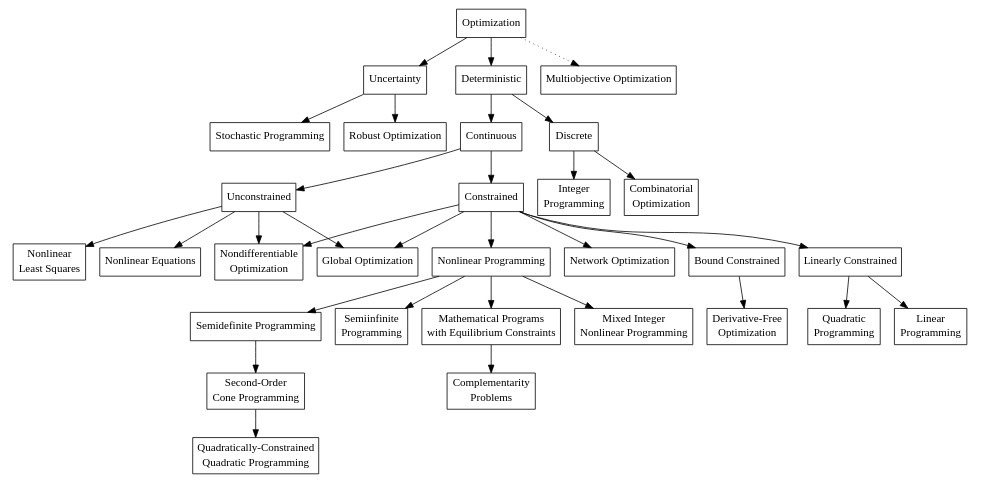
\includegraphics[width = \textwidth]{3_Methodology/otim.jpeg}
    \caption{``Taxonomia'' para problemas de otimização (fonte: ~\cite{neosguidetaxonomia})}
    \label{fig:taxonomia}
\end{figure}

\subsection{Introdução a Linguagem de Programação Matemática}

Linguagens de programação matemática são programas capazes de modelar interpretar o modelo matemático em um arquivo capaz de ser lido por \emph{solvers}, softwares com algoritmos para resolver problemas de otimização.

A sintaxe de uma linguagem de modelagem matemática é muito semelhante a modelagem algébrica, realizada de modo genérico é possível estender o modelo desenvolvido para outros problemas.

Os benefícios envolvendo o uso da linguagem estão relacionados ao fato de ser possível lidar com modelos algébricos, complexos e de larga escala, de maneira fácil e intuitiva que serão traduzidos em dados que podem ser processados por programas solucionadores.

Exemplos de problemas como descritos em \cite{Fourer2003AMPLProgramming} são:

\begin{itemize}
    \item Modelo de transporte \emph{multicommodity};
    
    \item Modelo de produção multiperiódico;
    
    \item Modelo de produção e transporte.
\end{itemize}

Os exemplos citados anteriormente são apenas uma parcela de uma infinidade de problemas de programação de larga escala.

A vantagem desse arranjo é que o mesmo modelo algébrico pode ser usado para resolver um problema de mesma natureza mas de tamanho diferente.

\subsection{AMPL}

O AMPL é uma linguagem procedural de modelagem algébrica cuja função é descrever e resolver problemas a partir do seu modelo matemático. 
A linguagem fora desenvolvida nos \emph{Bell Labs} por Robert Fourer, David Gay e Brian Kernighan com o intuito de ajudar as pessoas a comunicar modelos de otimização para sistemas de computação, aproveitando o poder e a conveniência de formulações algébricas familiares \cite{ampl}. 

Possui, atualmente, suporte para uma grande diversidade de \textit{solvers} tanto comerciais quanto código aberto.

A estrutura básica de um modelo em AMPL é da seguinte forma como mostrada em \cite{taha2008pesquisa}:

\begin{table}[H]
    \centering
    \caption{Estrutura de um modelo em AMPL}
    \begin{tabular}{|c|l|}
        \hline
        \multirow{4}{*}{Representação algébrica} & Definição dos conjuntos\\ & Definição dos parâmetros\\ & Definição das variáveis\\ & Representação do modelo\\ \hline
        \multirow{3}{*}{Implementação do modelo} & Dados de entrada\\ & Solução do modelo\\ & Apresentação dos resultados\\
        \hline
    \end{tabular}
    \label{tab:estrut_AMPL}
\end{table}

\subsection{Julia JuMP}

JuMP é uma linguagem de modelagem específica de domínio para otimização matemática incorporada em Julia~\cite{DunningHuchetteLubin2017}.
JuMP foi escrito puramente em Julia e possui código aberto, possuindo suporte para diversos \emph{solvers}, tanto comerciais quanto de código aberto.

Julia é uma linguagem de programação voltada para computação científica do tipo dinâmica criada no MIT.
A proposta da linguagem é suprir a falta de alta performance que geralmente acompanha as linguagens de dinâmicas.

De modo geral a linguagem Julia combina a velocidade de processamento semelhante a linguagens estáticas com os artifícios de linguagens dinâmicas tais como \emph{Python} e MATLAB.

\subsection{\emph{Solvers}}

\emph{Solvers}, como dito anteriormente, são programas que tem como finalidade buscar uma solução ótima baseada em um conjunto de parâmetros e podem ser tanto comerciais quanto constituídos de código aberto.
Ambas as categorias podem resolver determinados problemas de acordo com a natureza do sistema.


Um exemplo de \emph{solver} usado para resolver problemas de otimização linear e quadrática em variáveis contínuas e inteiras é o CEPLEX, \emph{solver} comercial baseado essencialmente em linguagem C cuja licença pertence à empresa IBM.
O suporte é fornecido para soluções de problemas quadráticos convexos, não convexos e restrições quadráticas convexas \cite{amplCEPLEX}. Os algoritmos usados são:

\begin{itemize}
    \item Problemas contínuos: primal e dual simplex, ponto interior;
    
    \item Problemas de números inteiros: \textit{branch and bound}, heurísticas de viabilidade e geradores de corte.
\end{itemize}

Outro exemplo de \emph{solver}, esse utilizado para solução de problemas de otimização não lineares, é o KNITRO.
O KNITRO é um pacote de programas em C para resolver otimização não linear e não linear inteiro misto, uma particularidade do software foi a grande atenção dada ao desempenho dos algoritmos KNITRO em classes mais simples de problemas, como sistemas de equações não-lineares e problemas irrestritos, uma vez que essas tarefas são cruciais na solução de problemas de programação não linear \cite{Byrd2006Knitro:Optimization}.
Segundo a Artelys, empresa responsável pelo software, o mesmo conta com os seguintes recursos para a solução de problemas de otimização, mostrados em \cite{knitroweb}:

\begin{itemize}
    \item Quatro algoritmos de ponto ativo/conjunto interno para problemas PNL;
    
    \item Três algoritmos para otimização discretas de problemas PNLIM;
    
    \item restrições de complementaridade para problemas de equilíbrio.
\end{itemize}

A entrada de um \emph{solver} para solução de problemas PNLIM, pode ser tomado como exemplo o manual disponível no NEOS-server como mostrado em \cite{neosguide}.

\begin{tcolorbox}[colback=white!10,title =\textbf{Dados de entrada de um \emph{solver}}]
    \begin{minipage}{\dimexpr\textwidth-\shadowsize-2\fboxrule-2\fboxsep-8pt}
    
    \begin{center}
        Min: $f(x,y)$   
    \end{center}

    \hspace{2cm}Sujeito a: 

    \begin{align*}
        c_{i}(x,y) = 0 \qquad \forall i&\in E\\
        c_{i}(x,y) \leq 0 \qquad \forall i&\in I\\
        x \qquad &\in X\\
        y \qquad &\in Y \quad \text{inteiro}
    \end{align*}
    \end{minipage}
    
    \vspace{1cm}
    
    Onde cada $c_{i}(x,y)$ é um mapeamento de $R^n \to R$, e $E$ e $I$ são conjuntos de índices para restrições de igualdades e desigualdades respectivamente. Tipicamente, as funções $f$ e $c_{i}$ têm algumas propriedades de suavidade, isto é, uma ou duas vezes continuamente diferenciáveis.
\end{tcolorbox}

\subsection{Hipóteses e definições da formulação do problema}

\begin{figure}[H]
    \centering
    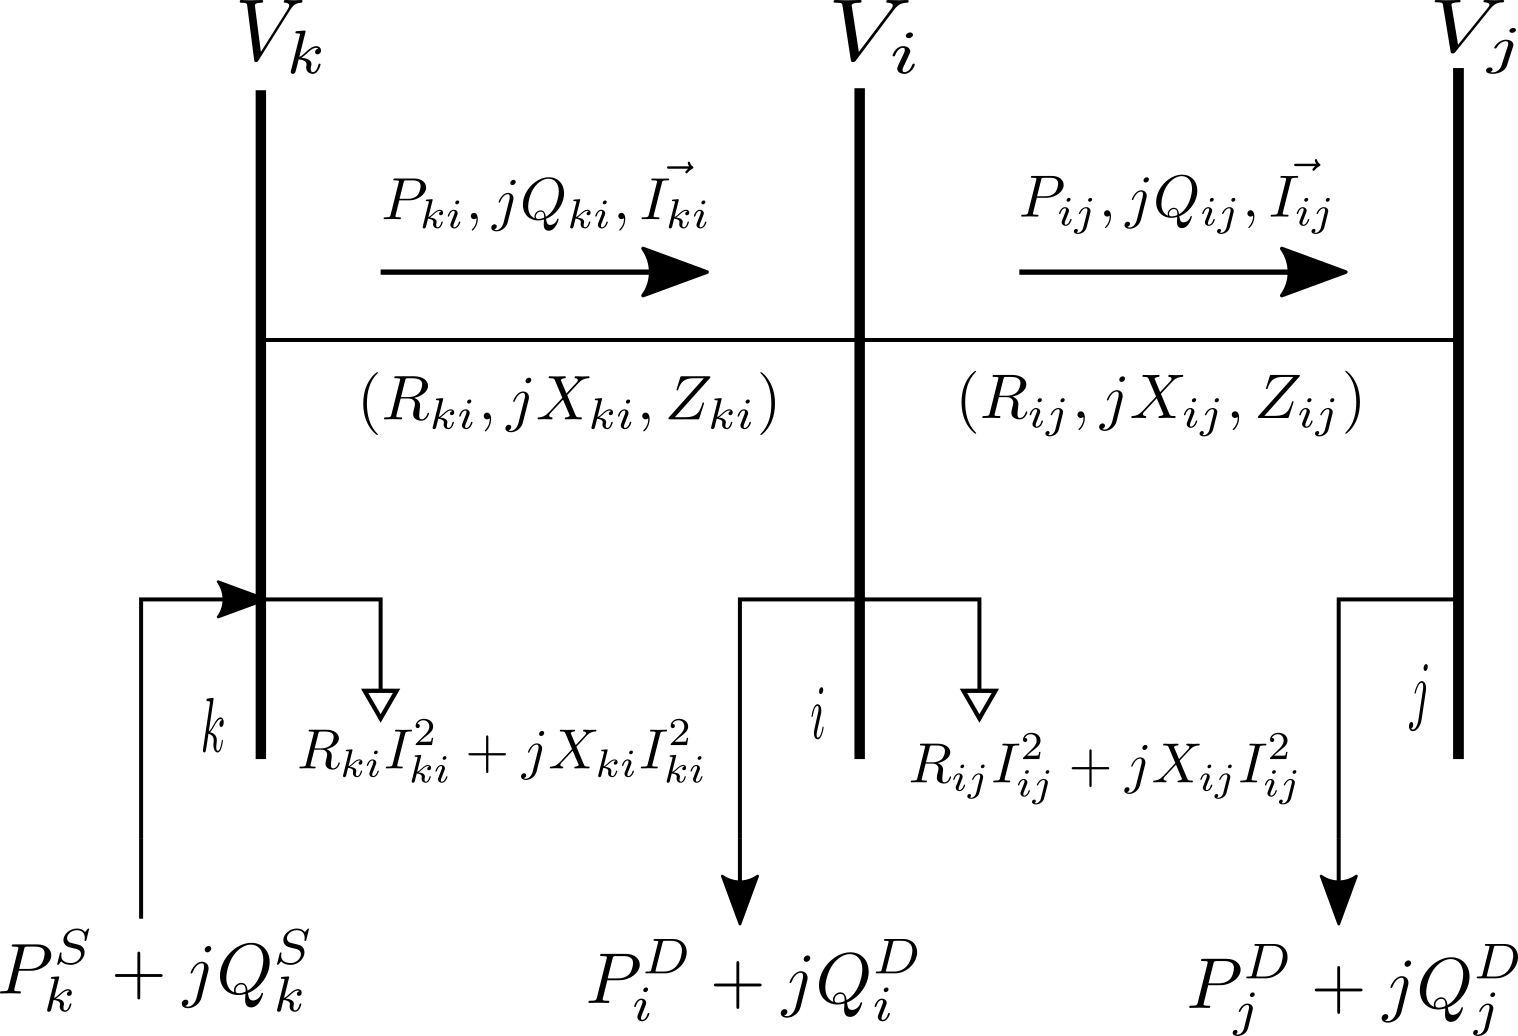
\includegraphics[width=0.7\textwidth]{3_Methodology/diagrama_nos.png}:
    \caption{Sistema de distribuição (Representação em barras)}
    \label{fig:SDR}
\end{figure}

Hipóteses adotadas:
Visando representar o funcionamento em regime permanente de um sistema de distribuição de energia, são feitas as seguintes hipóteses (comumente usadas nas formulações de varredura de fluxo de carga \cite{Shirmohammadi1988ANetworks} e mostradas na figura \ref{fig:SDR}):

\begin{itemize}
    \item As demandas das cargas na rede de distribuição são representadas como potência ativa e reativas constantes;

    \item O sistema é balanceado e representado pelo seu equivalente monofásico;
    
    \item As perdas de potência ativa e reativa no circuito \textit{ij} estão concentradas no nó \textit{i};
    
    \item As chaves são representadas como curtos circuitos de impedância nula.
\end{itemize}

\subsection{Modelo de otimização}

O modelo de otimização para RSD interpretado pelo AMPL possui a seguinte forma:

\begin{tcolorbox}[colback=white!10,title =\textbf{Modelo de um problema de otimização para RDS}]
    \begin{minipage}{\dimexpr\textwidth-\shadowsize-2\fboxrule-2\fboxsep-8pt}
    
    \begin{center}
        Minimizar: Função objetivo        
    \end{center}

    \hspace{2cm}Sujeito a:

    \begin{center}
        Restrições físicas\\
        Restrições operativas\\
    \end{center}
    \end{minipage}
\end{tcolorbox}


As restrições do problema devem ser tais que modelem as leis da física que regem um sistema de distribuição de energia elétrica e as faixas com as quais essas grandezas podem operar ao longo da rede.
Para isso define-se dois conjuntos de restrições, restrições físicas e restrições operativas.
\section{Modelagem do problema}

O problema de RSD envolve restrições não lineares e variáveis quadráticas, a fim de, em um primeiro momento, realizar uma tentativa de linearização e simplificação do problema, propõe-se uma mudança de variável que será aplicado nas equações ao longo deste documento.

\begin{align}
    I_{ij}^{sqr} = I_{ij}^{2}\;\forall ij \in \Omega_l \text{ e } V_{i}^{sqr} = V_{i}^{2}\; \forall i\in\Omega_b 
    \label{eq:change_variable}
\end{align}

%Explicar o significado de conjunto de circuitos e conjunto de nós do sistema


\subsection{Função objetivo}

Dado o modelo de otimização a ser interpretado pela linguagem de modelagem, é possível definir a função objetivo com base na figura~\ref{fig:SDR}.
A fim de reduzir as perdas ôhmicas na rede elétrica, a função objetivo do problema consiste em minimizar a somatória das perdas por resistência elétrica no conjunto de circuitos do sistema.

Definindo $c^{lss}$ como parâmetro que representa o custo das perdas de potência ativa na rede têm-se:

\begin{equation}
    \begin{split}
        \text{Min} = & c^{lss}\sum_{ij\in\Omega_{l}}R_{ij}I_{ij}^{2}\\
        = & c^{lss}\sum_{ij\in\Omega_{l}}R_{ij}I_{ij}^{sqr}
    \end{split}
    \label{eq:funcobjetivo}
\end{equation}

Tal que $\Omega_{l}$ é o conjunto de circuitos do sistema.
\subsection{Balanço de potência}

\begin{figure}[H]
    \centering
    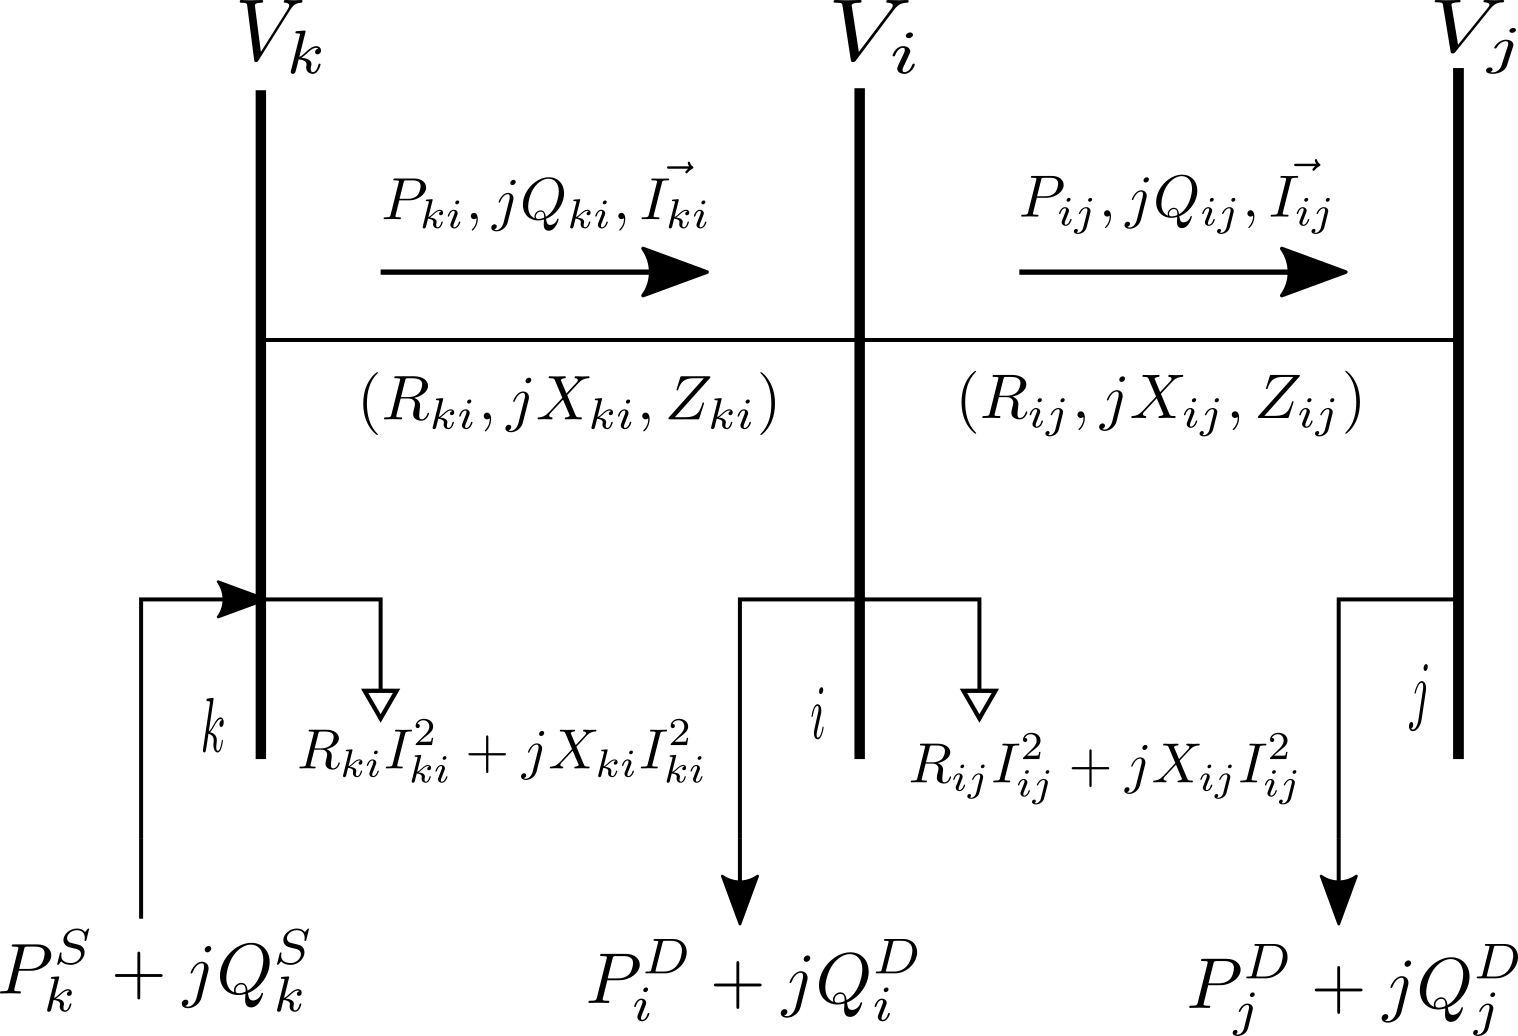
\includegraphics[width=0.6\textwidth]{3_Methodology/diagrama_nos.png}
    \caption{Exemplo de um diagrama de balanço de potência entre nós de um sistema de distribuição de energia elétrica}
    \label{fig:balanco_pot}
\end{figure}

A figura~\ref{fig:balanco_pot} representa a forma expandida da figura~\ref{fig:SDR}, para melhor compreensão do problema de balanço de potência, onde $m$ e $n$ representam um número qualquer de nós ligados ao nó $i$. 
Para isso considere que nos parâmetros e variáveis que representam um ramo, o primeiro subíndice representa o nó de partida e o segundo subíndice representa o nó de chegada (exemplo: $P_{12}$ se refere ao fluxo de potência ativa que vai do nó 1 para o nó 2).

Seja $P_{i}^{D}$ e $Q_{i}^{D}$ potência ativa e reativa demandada no nó i respectivamente e $P_{i}^{S}$ e $Q_{i}^{S}$ potência ativa e reativa gerada no nó $i$ respectivamente, têm-se que:

\begin{equation*}
    \sum_{ki\in\Omega_{l}}P_{ki} - \sum_{ij\in\Omega_{l}}(P_{ij} + R_{ij}I_{ij}^{2}) + P_{i}^{S} = P_{i}^{D}\quad\forall i \in\Omega_{b}
\end{equation*}

\begin{equation*}
    \sum_{ki\in\Omega_{l}}Q_{ki} - \sum_{ij\in\Omega_{l}}(Q_{ij} + X_{ij}I_{ij}^{2}) + Q_{i}^{S} = Q_{i}^{D}\quad\forall i \in\Omega_{b}
\end{equation*}

Dado que $\Omega_{b}$ é o conjunto de nós do sistema.
É possível mudar a variável \textit{k} pela variável \textit{j}, uma vez que ambas pertencem ao conjunto $\Omega_{l}$ e os somatórios envolvendo-as estão desconectadas, desse modo:
%desconectadas -> desconectados (para concordar com "somatórios")

\begin{equation}
    \sum_{ji\in\Omega_{l}}P_{ji} - \sum_{ij\in\Omega_{l}}(P_{ij} + R_{ij}I_{ij}^{2}) + P_{i}^{S} = P_{i}^{D}\quad\forall i \in\Omega_{b}\label{eq:fluxo_pot_ativa}  
\end{equation}


\begin{equation}
    \sum_{ji\in\Omega_{l}}Q_{ji} - \sum_{ij\in\Omega_{l}}(Q_{ij} + X_{ij}I_{ij}^{2}) + Q_{i}^{S} = P_{i}^{D}\quad\forall i \in\Omega_{b}\label{eq:fluxo_pot_reativa}
\end{equation}

O sistema de equações não lineares em \ref{eq:fluxo_pot_ativa} e \ref{eq:fluxo_pot_reativa} representam a operação em regime permanente de uma rede elétrica radial e são frequentemente utilizados no método de varredura de fluxo de carga \cite{Shirmohammadi1988ANetworks} e \cite{Cespedes1990NewNetworks}.
\subsection{Queda de tensão entre nós}


O conjunto de equações a seguir mostram o caso típico de formulação do problema de fluxo de carga para redes elétricas radiais.

Da figura \ref{fig:SDR}, a queda de tensão do circuito é definida pela equação \ref{eq:queda_tensao}.

\begin{equation}
    \Vec{V}_{i} - \Vec{V}_{j} = I_{ij}(R_{ij} + jX_{ij})\quad\forall i,j \in \Omega_{l}
    \label{eq:queda_tensao}
\end{equation}

Em que $\Omega_{l}$ é o conjunto de circuitos, ou seja, o conjunto de todos os nós do sistema.

Através da fórmula para o cálculo da potência aparente, $I_{ij}$ pode ser calculado usando a equação \ref{eq:corrente_ramo}.

\begin{equation}
    I_{ij} = \left(\frac{P_{ij} + jQ_{ij}}{\Vec{Vj}}\right)^{*}\quad\forall ij \in \Omega_{l}
    \label{eq:corrente_ramo}
\end{equation}

Substituindo $I_{ij}$ da equação \ref{eq:corrente_ramo} na equação \ref{eq:queda_tensao} obtém-se a equação \ref{eq:queda_tensao_pot} que define a queda de tensão em função das potências e impedâncias do circuito.


Seja $(P_{ij} + jQ_{ij})^{*} = (P_{ij} - jQ_{ij})$, logo:

\begin{equation}
    (\Vec{V}_{i} - \Vec{V}_{j})\Vec{V}_{j}^{*} = (P_{ij} - jQ_{ij})(R_{ij} + jX_{ij}) \quad\forall ij \in \Omega_{l}
    \label{eq:queda_tensao_pot}
\end{equation}

Considerando que $\Vec{V}_{i} = V_{i}\angle{\theta_{i}}$, $\Vec{V}_{j} = V_{j}\angle{\theta_{j}}$ e $\theta_{ij} = \theta_{i} - \theta_{j}$, tal que  $V_{i}$ e $V_{j}$ representam as magnitudes da tensão em seus respectivos nós bem como $\theta_{i}$ e $\theta_{j}$ representam seus ângulos.
Dessa forma a equação \ref{eq:queda_tensao_pot} pode ser escrita decompondo a fase de suas exponenciais, como mostra a equação \ref{eq:queda_tensao_sencos}.

\begin{equation}\label{eq:queda_tensao_sencos}
    V_{i}V_{j}[cos\theta_{ij} + jsen\theta_{ij}] - V_{j}^{2} = (P_{ij} - jQ_{ij})(R_{ij} + jX_{ij}) \quad\forall ij \in \Omega_{l}
\end{equation}

Identificando as partes real e imaginária na equação \ref{eq:queda_tensao_sencos}, obtém-se:

\begin{equation}
    V_{i}V_{j}cos\theta_{ij} = V_{j}^{2} + (R_{ij}P_{ij} + X_{ij}Q_{ij})\quad\forall ij \in \Omega_{l}
    \label{eq:queda_tensao_real}
\end{equation}

\begin{equation}
    V_{i}V_{j}sen\theta_{ij} = X_{ij}P_{ij} - R_{ij}Q_{ij}\quad\forall ij \in \Omega_{l}
    \label{eq:queda_tensao_imaginaria}
\end{equation}

Usando a fórmula da trigonometria, que é a relação básica entre o seno e o cosseno, $sen^{2}(\theta_{ij}) + cos^{2}(\theta_{ij}) = 1$, e somando os quadrados das equações \ref{eq:queda_tensao_real} e \ref{eq:queda_tensao_imaginaria}, obtém-se:

\begin{equation}
    V_{i}^{2} - 2(R_{ij}P_{ij} + X_{ij}Q_{ij}) - Z_{ij}^{2}I_{ij}^{2} - V_{j}^{2} = 0\quad\forall ij \in \Omega_{l}
    \label{eq:queda_tensao_restricao}
\end{equation}

Nota-se que a equação \ref{eq:queda_tensao_restricao} não depende da diferença angular entre as tensões, e é possível obter a magnitude da tensão do nó ($V_j$) em termos da magnitude inicial ($V_i$), o fluxo de potência ativa ($P_{ij}$), o fluxo de potência reativa ($Q_{ij}$), a magnitude do fluxo de corrente ($I_{ij}$) e os parâmetros elétricos do ramo \textit{ij}.

\subsection{Fluxo de corrente em um ramo}

Na equação de queda de tensão, a magnitude do fluxo de corrente $I_{ij}$ é mostrada na equação \ref{eq:corrente_magnitude}, calculada a partir do produto com seu complexo conjugado.

\begin{equation}
    I_{ij}^{2} = \frac{P_{ij}^{2}+Q_{ij}^{2}}{V_{j}^{2}}\quad\forall ij \in \Omega_{l}
    \label{eq:corrente_magnitude}
\end{equation}

\subsection{Restrições operativas do sistema}

O problema de reconfiguração está sujeita a restrições operativas imposta pela agência reguladora, tais como limite de tensão, correntes tanto para o conjunto de ramos do sistema quanto para a operação das chaves.
Dessa forma é possível determinar as restrições operativas para o funcionamento do SDEE.

\subsubsection{Limites de tensão}

Em um sistema de distribuição de energia elétrica é preciso garantir que a tensão em um nó esteja dentro de uma faixa de operação determinada por norma, por isso uma restrição fundamental para o problema é a restrição de limites de tensão em um nó, determinada pela seguinte equação:

\begin{equation}
    \underline{V}^{2} \leq V_{i}^{sqr} \leq \overline{V}^{2}\qquad\forall i \in\Omega_{b}
\end{equation}

Onde $\underline{V}$ e $\overline{V}$ representam o limite inferior e superior de tensão, respectivamente, que uma rede pode possuir.


\subsubsection{Limite de corrente}

Assim como as tensões, o fluxo de corrente também deve ser limitado para não comprometer o SDEE.
Assim a equação que descreve a restrição é:

\begin{equation}
    0 \leq I_{ij}^{sqr} \leq \overline{I}_{ij}^{2} \qquad\forall ij\in\Omega_{l} 
\end{equation}

\subsubsection{Chaves presentes no sistema}

Para reconfiguração do SDEE, existem chaves ao longo da rede que podem ser modificadas de modo a garantir a operação desejada.
Considere as seguintes restrições:

\begin{figure}[H]
    \centering
    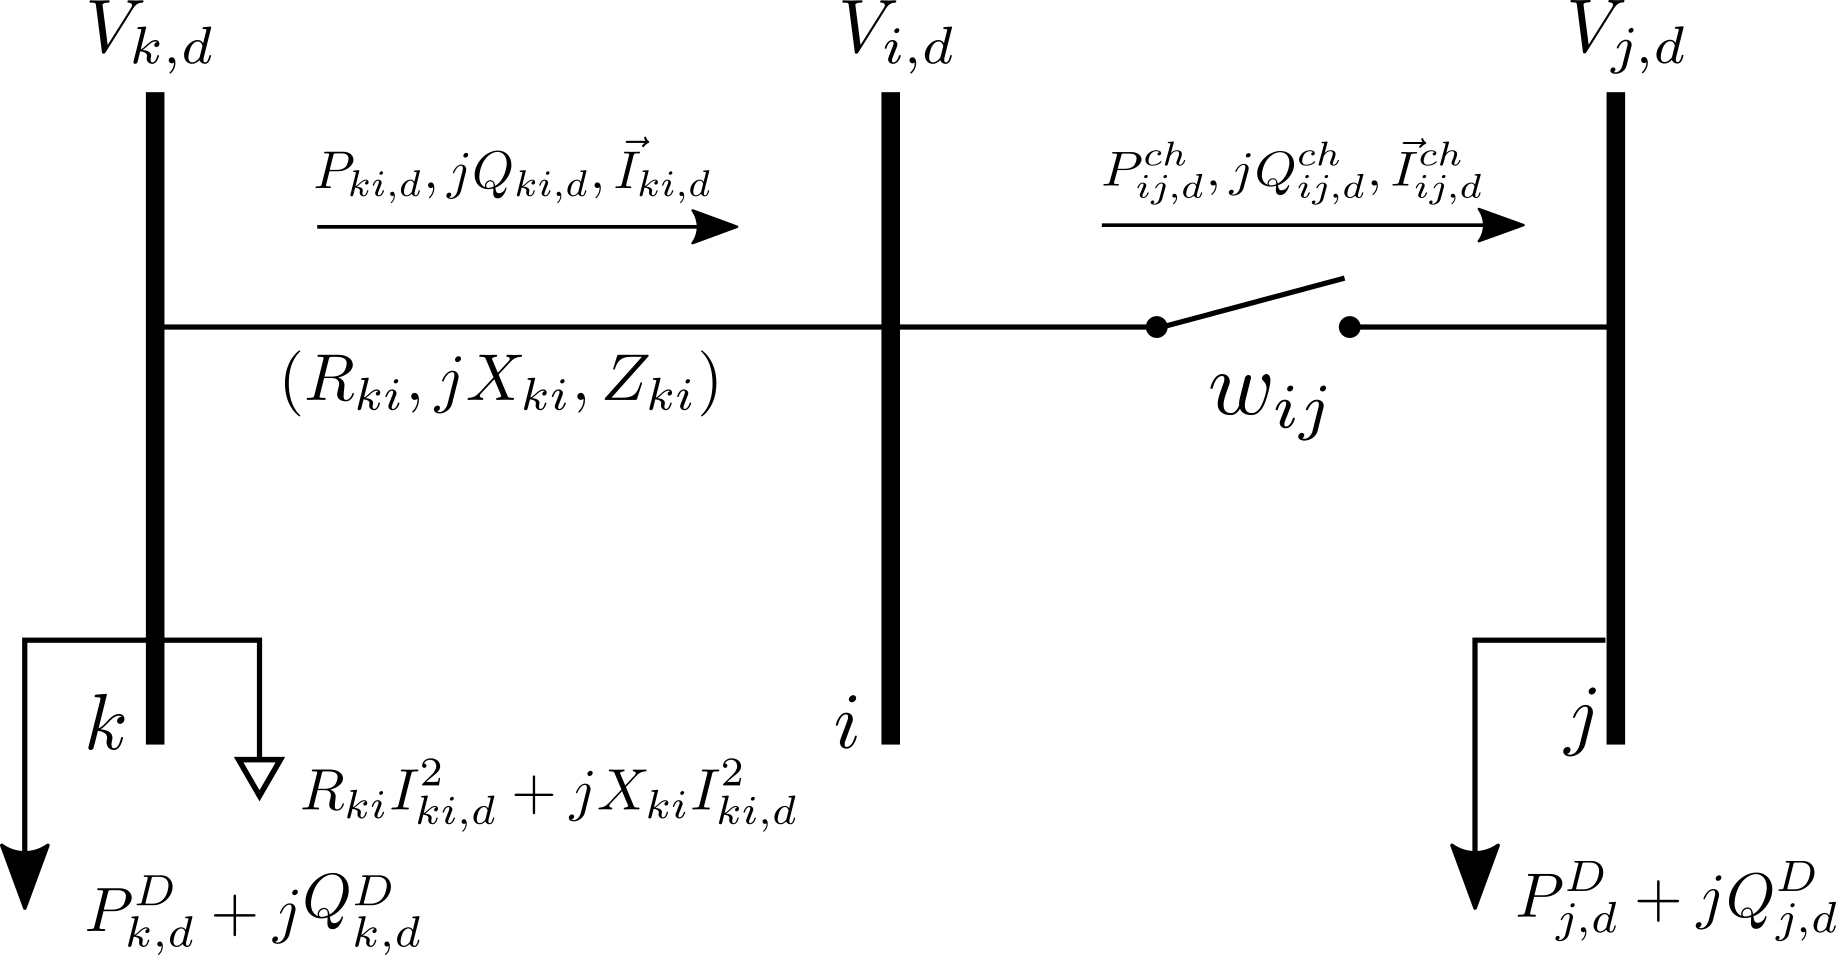
\includegraphics[scale = 1.3]{4_Modeling/diagrama_chaves.png}
    \caption{Modelo de uma chave conectada entre dois nós}
    \label{fig:diagrama_chave}
\end{figure}
    
\begin{itemize}
    \item Balanço de potência
\end{itemize}
    Com base na figura \eqref{fig:diagrama_chave}, faz-se necessário reformular as equações de balanço de potência, expressas em~\eqref{eq:fluxo_pot_ativa} e \eqref{eq:fluxo_pot_reativa}, adicionando as variáveis que representam as chaves na modelagem do problema.

\begin{equation}
    \sum_{ji\in\Omega_{l}}P_{ji} - \sum_{ij\in\Omega_{l}}(P_{ij} + R_{ij}I_{ij}^{sqr})+ \sum_{ji\in\Omega_{ch}}P_{ji}^{ch} -\sum_{ij\in\Omega_{ch}}P_{ij}^{ch} + P_{i}^{S} = P_{i}^{D}\quad\forall i \in\Omega_{b}\label{eq:fluxo_pot_ativa_chaves}  
\end{equation}
    
    
\begin{equation}
    \sum_{ji\in\Omega_{l}}Q_{ji} - \sum_{ij\in\Omega_{l}}(Q_{ij} + X_{ij}I_{ij}^{sqr})+ \sum_{ji\in\Omega_{ch}}Q_{ji}^{ch} -\sum_{ij\in\Omega_{ch}}Q_{ij}^{ch} + Q_{i}^{S} = P_{i}^{D}\quad\forall i \in\Omega_{b}
    \label{eq:fluxo_pot_reativa_chaves}
\end{equation}
    
Onde $\Omega_{ch}$ representa o conjunto de chaves da rede elétrica e $w_{ij}$ é uma variável binária que representa o estado da chave \textit{ij}: se $w_{ij} = 1$ a chave ij está fechada, caso contrário a chave está aberta, ver figura~\ref{fig:diagrama_chave}. $P_{ij}^{ch}$ e $Q_{ij}^{ch}$ representam o fluxo de potência ativa e reativa da chave \textit{ij}.

As restrições expressas nas equações \eqref{eq:fluxo_pot_ativa_chaves} e \eqref{eq:fluxo_pot_reativa_chaves} são extensões das equações \eqref{eq:fluxo_pot_ativa} e \eqref{eq:fluxo_pot_reativa}, considerando a presença de chaves na rede elétrica.
    
Além do balanço de potência, outras restrições devem ser estabelecidas devido à presença de chaves, são elas:

\begin{itemize}
    \item Diferença de tensões entre dois nós conectados por uma chave
\end{itemize}

    
A diferença de tensão entre nós, na presença de chaves, deve ser igual a zero, uma vez que, de acordo com as hipóteses adotadas, a impedância da chaves é representada como uma impedância nula.
Sendo assim, usando a variável binária $w_{ij}$ é possível equacionar a restrição da seguinte forma:

\begin{equation}
    -(\overline{V}^{2} - \underline{V}^{2})(1-w_{ij}) \leq V_{i}^{sqr} - V_{j}^{sqr} \leq (\overline{V}^{2} - \underline{V}^{2})(1-w_{ij})\qquad\forall ij\in\Omega_{ch}
\end{equation}
    
É possível observar que se $w_{ij}$ for igual a 1 (chave fechada), a diferença entre as tensões no nó $i$ e nó $j$ será igual a zero, o que condiz a hipótese adotada.

\begin{itemize}
   \item Fluxo de potência na chave
\end{itemize} 
    
O fluxo de potência na chave é determinada pelas equações abaixo.
    
\begin{equation}
    -(\overline{V}\,\overline{I}_{ij}^{ch})w_{ij} \leq P_{ij}^{ch} \leq (\overline{V}\,\overline{I}_{ij}^{ch})w_{ij}\qquad\forall ij\in\Omega_{ch}   
\end{equation}
    
    
\begin{equation}
    -(\overline{V}\,\overline{I}_{ij}^{ch})w_{ij} \leq Q_{ij}^{ch} \leq (\overline{V}\,\overline{I}_{ij}^{ch})w_{ij}\qquad\forall ij\in\Omega_{ch}   
\end{equation}
    
É possível notar que se a variável $w_{ij}$ for igual a 0 (chave aberta), o fluxo de potência na chave é igual a zero, o que condiz com a proposta do elemento de circuito na rede; quando igual a 1, as restrições representam o fluxo máximo de potência ativa e reativa permitida na chave quando está energizada.

\subsubsection{Restrição de radialidade}

A representação de um SDEE é feita através de nós e circuitos. Fazendo analogia com a teoria de grafos, um SDEE pode ser considerado como um grafo formado por n arcos e m nós.
Da teoria de grafos, uma árvore é um grafo conexo sem ciclos, assim é possível comparar a topologia radial de um SDEE com uma árvore.
Como mostrado em \cite{Bazaraa1990LinearFlows}, a árvore de um grafo é um sub-grafo com ($m-1$) arcos.

Assim, pode-se dizer que a topologia de um SDEE com $n_{b}$ nós é radial se satisfaz as duas seguintes condições: Condição 1: a solução deve apresentar ($n_{b}$) circuitos; e Condição 2: a solução deve gerar uma topologia conexa. Observa-se que a restrição de radialidade tem que ser formada pelas condições 1 e 2.
Somente a condição 1 não garante a radialidade do SDEE. 

O problema de RSD cumpre com as seguintes características: 1) apenas uma única subestação existente no SDEE (nó da subestação); 2) todos os outros nós são nós de carga; 3) a primeira lei de kirchhoff, deve ser cumprida, e 4) o objetivo é encontrar a melhor topologia radial. 
A condição 1 é satisfeita pela seguinte restrição:

\begin{equation}
    |\Omega_{l}| + \sum_{ij\in\Omega_{ch}}w_{ij} = |\Omega_{b}| - 1
    \label{eq:radialidade}
\end{equation}

Em que $|\Omega|$ é um operador que calcula o número de elementos do conjunto $\Omega$.

Uma solução que satisfaz a restrição de balanço de potência (primeira Lei de Kirchhoff) tem de fornecer a demanda de potência em cada nó de carga de modo que exista um caminho entre a subestação e os nós de carga. Portanto, cada nó está ligado com a subestação, formando um grafo conexo, o que comprova a Condição 2. 
Assim, quando as restrições de balanço de potência são combinadas com a Condição 1, cada nó de carga está ligado por um único caminho com a subestação, isto é, o SDEE é conexo, sem malhas.

\begin{figure}[H]
    \centering
    
\includegraphics[scale = 0.8]{4_Modeling/restricao_fail.png}
    \caption{Exemplo de rede não radial que obedece a equação \eqref{eq:radialidade}}
    \label{fig:radialidade_wrong}
\end{figure}

Observa-se que a figura \ref{fig:radialidade_wrong}, embora respeite a equação \eqref{eq:radialidade} (5 ramos para 6 nós), não é uma topologia radial. Isso pode acontecer se e somente se a equação~\eqref{eq:radialidade} for levada em consideração.

\begin{figure}[H]
    \centering
    
\includegraphics[scale=0.6]{4_Modeling/restricao_radialidade.png}
    \caption{Exemplo de rede radial que obedece a equação \eqref{eq:radialidade}}
    \label{fig:radialidade_right}
\end{figure}

Observe agora a figura \ref{fig:radialidade_right}, note que ela é uma topologia radial, como dito anteriormente é necessário duas condições para garantir tal configuração, como no problema já existem equações que garantem a primeira Lei de Kirchhoff, a topologia final será radial. 
É possível notar que todos os nós estão interligados, direto e não direto, com o nó 1 (nó da subestação).
Isso acontece pois as equações de balanço de potência obrigam que haja fluxo de potência para atender as demandas dos mesmos.

Assim a equação \eqref{eq:radialidade} junto com \eqref{eq:fluxo_pot_ativa_chaves} e \eqref{eq:fluxo_pot_reativa_chaves} fornecem as condições necessárias para e suficientes para garantir uma topologia final radial \cite{Lavorato2012ImposingProblems}.


\section{Formulação dos problemas de programação}

Como dito anteriormente, este trabalho tem como objetivo analisar o problema de RSD como um problema de otimização.
As equações já descritas são suficientes para descrever o problema e, em conjunto, formam um problema de programação não linear (como mostra a seção seguinte) que posteriormente foram convertida em problemas de outras naturezas.
\subsection{Problema de programação não linear}

Utilizando a metodologia descrita anteriormente, é possível modelar o problema de reconfiguração de redes radiais, utilizando as equações~\ref{eq:funcobjetivo}, \ref{eq:fluxo_pot_ativa_chaves}, \ref{eq:fluxo_pot_reativa_chaves}, \ref{eq:corrente_ramo} da seguinte forma:


\begin{tcolorbox}[enhanced jigsaw,breakable,pad at break*=1mm,colback=white!10,title =\textbf{Problema de PLIM para RSD}]

\begin{align*}\label{eq:NL_funcobj}
    \text{Min}\quad c^{lss}\sum_{ij\in\Omega_l}R_{ij}I_{ij}^{sqr}
\end{align*}

Sujeito a:

\begin{equation*}\label{eq:NL_PA}
    \sum_{ji\in\Omega_{l}}P_{ji} - \sum_{ij\in\Omega_{l}}(P_{ij} + R_{ij}I_{ij}^{sqr})+ \sum_{ji\in\Omega_{ch}}P_{ji}^{ch} -\sum_{ij\in\Omega_{ch}}P_{ij}^{ch} + P_{i}^{S} = P_{i}^{D}\quad\forall i \in\Omega_{b}  
\end{equation*}

\begin{equation*}\label{eq:NL_PR}
    \sum_{ji\in\Omega_{l}}Q_{ji} - \sum_{ij\in\Omega_{l}}(Q_{ij} + X_{ij}I_{ij}^{sqr})+ \sum_{ji\in\Omega_{ch}}Q_{ji}^{ch} -\sum_{ij\in\Omega_{ch}}Q_{ij}^{ch} + Q_{i}^{S} = Q_{i}^{D}\quad\forall i \in\Omega_{b}
\end{equation*}

\begin{equation*}\label{eq:NL_voltage}
    V_{i}^{sqr} - 2(R_{ij}P_{ij} + X_{ij}Q_{ij}) - Z_{ij}^{2}I_{ij}^{sqr} - V_{j}^{sqr} = 0\quad\forall ij \in \Omega_{l}
\end{equation*}

\begin{equation*}\label{eq:NL_power}
    V_{j}^{sqr}I_{ij}^{sqr} = P_{ij}^{2}+Q_{ij}^{2}\quad\forall ij \in \Omega_{l}
\end{equation*}

\begin{equation*}\label{eq:NL_voltagekeys}
    -(\overline{V}^{2} - \underline{V}^{2})(1-w_{ij}) \leq V_{i}^{sqr} - V_{j}^{sqr} \leq (\overline{V}^{2} - \underline{V}^{2})(1-w_{ij})\qquad\forall ij\in\Omega_{ch}
\end{equation*}
    
\begin{equation*}\label{eq:NL_PAkeys}
    -(\overline{V}\,\overline{I}_{ij}^{ch})w_{ij} \leq P_{ij}^{ch} \leq (\overline{V}\,\overline{I}_{ij}^{ch})w_{ij}\qquad\forall ij\in\Omega_{ch}
\end{equation*}
    
    
\begin{equation*}\label{eq:NL_PRkeys}
    -(\overline{V}\,\overline{I}_{ij}^{ch})w_{ij} \leq Q_{ij}^{ch} \leq (\overline{V}\,\overline{I}_{ij}^{ch})w_{ij}\qquad\forall ij\in\Omega_{ch}   
\end{equation*}
    
\begin{equation*}\label{eq:NL_radialidade}
    |\Omega_{l}| + \sum_{ij\in\Omega_{ch}}w_{ij} = |\Omega_{b}| - 1
\end{equation*}

\begin{equation*}\label{eq:NL_limvoltage}
    \underline{V}^{2} \leq V_{i}^{sqr} \leq \overline{V}^{2}\qquad\forall i \in\Omega_{b}
\end{equation*}

\begin{equation*}\label{eq:NL_limcurrent}
    0 \leq I_{ij}^{sqr} \leq \overline{I}_{ij}^{2} \qquad\forall ij\in\Omega_{l} 
\end{equation*}

\begin{equation*}\label{eq:NL_binario}
    w_{ij}\quad\text{binário}\qquad\forall ij \in\Omega_{ch}
\end{equation*}
\end{tcolorbox}

O problema descrito no conjunto equações destacadas é considerado um problema de programação não linear devido à presença da restrição expressa na equação~\ref{eq:NL_power}, uma vez que ela é o produto de duas variáveis que representam tensão e corrente do sistema ($V_{j}^{sqr}$ e $I_{ij}^{sqr}$) que são iguais a soma dos quadrados das variáveis que representam as potências ativas e reativas do sistema ($P_{ij}$ e $Q_{ij}$).

\subsection{Problema de programação cônica de segunda ordem}

O problema de PNLIM pode ser convertido em um problema convexo. Relaxando a restrição não linear do problema, pode-se transformar o problema de PNLIM em um problema de programação cônica de segunda ordem inteiro misto (PCSOIM).

Em~\cite{Romais2014ReconfiguracaoMista}, é possível escrever um problema de otimização cônica em um problema de programação linear, que contenha pelo menos uma restrição cônica. 
Uma restrição cônica 
\subsection{Problema de programação linear}

Utilizando algumas aproximações, o problema de programação não linear inteiro misto pode ser convertido em um problema de programação linear inteiro misto.

Inicialmente pode-se aproximar o quadrado da tensão em um nó do circuito como o quadrado da tensão nominal.
Esta simplificação é valida e com um erro de aproximação baixo, devido ao intervalo restrito da magnitude de tensão [$\underline{V}^2$,$\overline{V}^2$] e comprovado experimentalmente depois de realizar varias simulações apresentadas em~\cite{Goncalves2013ModelosRadiais} e \cite{Alves2012Alocacao-}.
Dessa forma o primeiro termo da equação~\eqref{eq:PNLIM_power} pode ser reescrita da seguinte forma:

\begin{equation}\label{eq:L_powervoltage}
    V_{j}^{2}I_{ij}^{sqr} \approx (V^{\text{nom}})^{2}I_{ij}^{sqr}\qquad\forall ij\in\Omega_{l}
\end{equation}

Da equação~\eqref{eq:L_powervoltage}, é possível perceber que não existe mais produto entre variáveis, visto que $V^{nom}$ é um parâmetro e, portanto, uma constante do problema.

O outro passo é linearizar os termos $P_{ij}^2$ e $Q_{ij}^2$, o que é possível, utilizando o método de linearização por partes como mostrado em~\cite{Goncalves2013ModelosRadiais} e \cite{Alves2012Alocacao-}.

O método de linearização por partes consiste em uma somatória de segmentos de retas a partir de blocos discretos igualmente espaçados.
A figura~\ref{fig:linearization} mostra a discretização do módulo de uma variável pelo seu quadrado.

\begin{figure}[H]
    \centering
    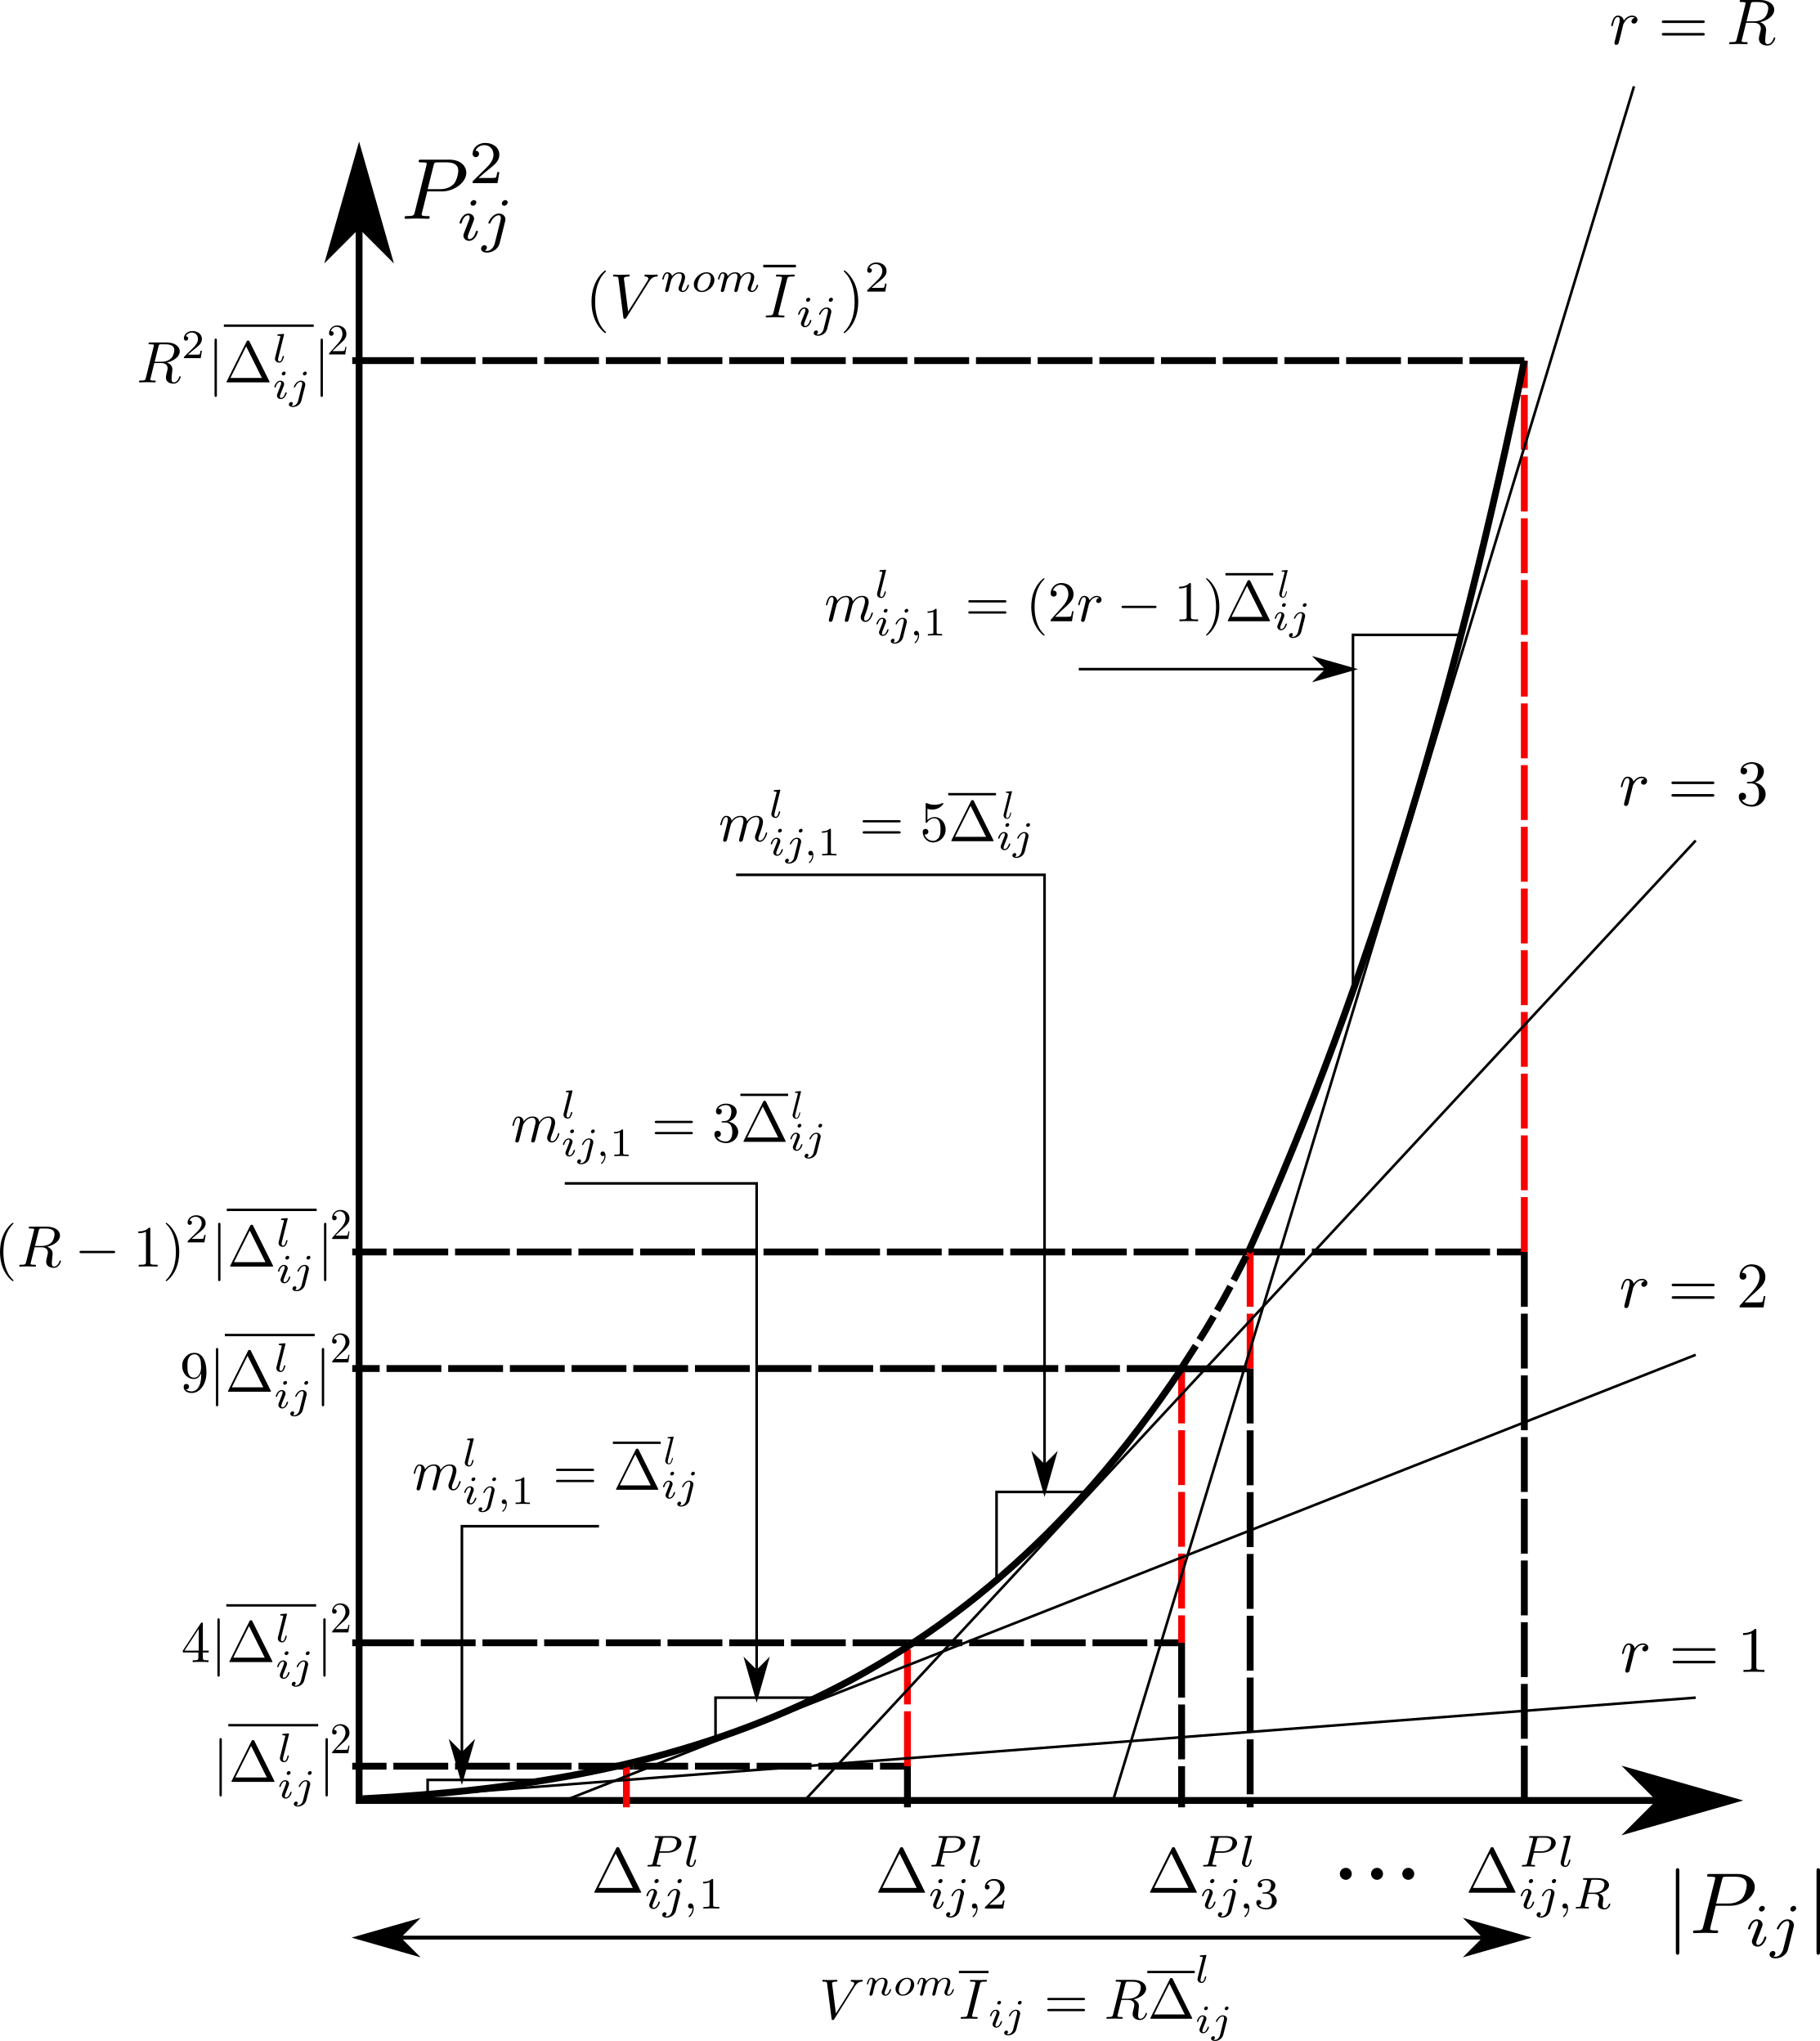
\includegraphics[width = 0.6\textwidth]{5_Formulation/lin.png}
    \caption{Linearização da potência ativa pelo método de linearização por partes}
    \label{fig:linearization}
\end{figure}{}

Com base na figura~\ref{fig:linearization}, o valor de $P_{ij}^{2}$ pode ser descrito como o somatório dos catetos paralelos ao eixo da ordenada (segmentos em vermelho), a mesma analogia pode ser feita com $Q_{ij}^{2}$, resultando na equação~\eqref{eq:Lin_quadpower}.

\begin{equation}\label{eq:Lin_quadpower}
    P_{ij}^2 + Q_{ij}^2 \approx \sum_{r = 1}^{R}m_{ij,r}^{l}\Delta_{ij,r}^{Pl} + \sum_{r = 1}^{R}m_{ij,r}^{l}\Delta_{ij,r}^{Ql} \qquad\forall ij\in\Omega_{l} 
\end{equation}

Tal que $\Delta_{ij,r}^{Pl}$ e $\Delta_{ij,r}^{Ql}$ são variáveis que representam o r-ésimo bloco de $P_{ij}$ e $Q_{ij}$ do circuito $ij$ respectivamente, as quais devem obedecer a seguinte restrição:

\begin{equation}\label{eq:Lin_Pdeltalim}
    0 \leq \Delta_{ij,r}^{Pl} \leq \overline{\Delta}_{ij,r}^l \qquad\forall ij\in\Omega_{l} 
\end{equation}

\begin{equation}\label{eq:Lin_Qdeltalim}
    0 \leq \Delta_{ij,r}^{Ql} \leq \overline{\Delta}_{ij,r}^l \qquad\forall ij\in\Omega_{l} 
\end{equation}

O parâmetro $\Delta_{ij}^{l}$ representa o valor máximo do bloco de discretização, assim dado um valor $R$ de discretizações, pode-se determinar $\Delta_{ij}^{l}$ como o quociente entre o módulo da potência aparente máxima e a quantidade de discretizações $R$, obtendo assim a equação~\eqref{eq:Lin_maxdelta}.

\begin{equation}\label{eq:Lin_maxdelta}
    \overline{\Delta}_{ij}^{l} = \frac{V^{\text{nom}}\overline{I}_{ij}}{R} \qquad\forall ij\in\Omega_{l} 
\end{equation}

$m_{ij,r}^{l}$ representa a inclinação do r-ésimo bloco de potência ativa e reativa no circuito $ij$ e é descrito pela equação~\eqref{eq:Lin_m}.

\begin{equation}\label{eq:Lin_m}
    \begin{split}
        m_{ij,r}^{l} & = \frac{r^2|\overline{\Delta_{ij}^{l}}|^2 - (r-1)^2|\overline{\Delta_{ij}^{l}}|^2}{|\overline{\Delta_{ij}^{l}}|}\qquad\forall ij\in\Omega_{l}\\
        & = |\overline{\Delta_{ij}^{l}}|(r^2 - r^2 + 2r - 1)\qquad\quad\forall ij\in\Omega_{l}\\
        & = (2r-1)\overline{\Delta_{ij}^{l}}\qquad\qquad\qquad\qquad\forall ij\in\Omega_{l}
    \end{split}
\end{equation}

Para que se possa implementar a linearização descrita pelas equações anteriores é preciso modelar o módulo das variáveis $P_{ij}$ e $Q_{ij}$. Isto pode ser feito utilizando duas variáveis positivas de tal modo que:

\begin{equation}\label{eq:Lin_PQmod}
    \begin{split}
        P_{ij} = P_{ij}^{+} - P_{ij}^{-} & \qquad\forall ij\in\Omega_{l}\\
        Q_{ij} = Q_{ij}^{+} - Q_{ij}^{-} & \qquad\forall ij\in\Omega_{l}
    \end{split}
\end{equation}

\begin{equation}
    \begin{split}
        0 \leq P_{ij}^{+} & \qquad\forall ij\in\Omega_{l}\\
        0 \leq P_{ij}^{-} & \qquad\forall ij\in\Omega_{l}\\
        0 \leq Q_{ij}^{+} & \qquad\forall ij\in\Omega_{l}\\
        0 \leq Q_{ij}^{-} & \qquad\forall ij\in\Omega_{l}
    \end{split}
\end{equation}

Aplicando o módulo em $P_{ij}$ e $Q_{ij}$, obtém-se:

\begin{equation}\label{eq:Lin_modPA}
        |P_{ij}| = P_{ij}^{+} + P_{ij}^{-} = \sum_{r = 1}^{R}\Delta_{ij,r}^{Pl}  \qquad\forall ij\in\Omega_{l}
\end{equation}

\begin{equation}\label{eq:Lin_modPR}
        |Q_{ij}| = Q_{ij}^{+} + Q_{ij}^{-} = \sum_{r = 1}^{R}\Delta_{ij,r}^{Ql}  \qquad\forall ij\in\Omega_{l}
\end{equation}

Por fim, o problema de programação linear inteiro misto pode ser descrito no seguinte formato:


\begin{tcolorbox}[breakable,pad at break*=1mm,colback=white!10,title =\textbf{Problema de PLIM para RSD}]

\begin{equation}\label{eq:plim}
\left.
    \begin{tabular}{ll}
               & Min ~\eqref{eq:PNLIM_funcobj}\\
    Sujeito a: &\eqref{eq:PNLIM_fluxoP} - \eqref{eq:PNLIM_voltage}, \eqref{eq:PNLIM_voltagekeys} - \eqref{eq:PNLIM_currentlim} \textbf{(Equações já propostas para RSD)}\\
    &\textbf{(Bloco de equações para linearização de~\eqref{eq:PNLIM_power})}\\
    &$(V^{nom})^{2}I_{ij}^{sqr} = \sum_{r = 1}^{R}m_{ij,r}^{l}\Delta_{ij,r}^{Pl} + \sum_{r = 1}^{R}m_{ij,r}^{l}\Delta_{ij,r}^{Ql} \qquad\forall ij\in\Omega_{l}$ \\
    &$P_{ij} = P_{ij}^{+} - P_{ij}^{-}\qquad\forall ij\in\Omega_{l}$\\
    &$Q_{ij} = Q_{ij}^{+} - Q_{ij}^{-}\qquad\forall ij\in\Omega_{l}$\\
    & $P_{ij}^{+} + P_{ij}^{-} = \sum_{r = 1}^{R}\Delta_{ij,r}^{Pl}  \qquad\forall ij\in\Omega_{l}$\\
    & $Q_{ij}^{+} + Q_{ij}^{-} = \sum_{r = 1}^{R}\Delta_{ij,r}^{Ql}  \qquad\forall ij\in\Omega_{l}$\\
    & $0 \leq \Delta_{ij,r}^{Pl} \leq \overline{\Delta}_{ij,r}^l \qquad\forall ij\in\Omega_{l}$\\
    & $0 \leq \Delta_{ij,r}^{Ql} \leq \overline{\Delta}_{ij,r}^l \qquad\forall ij\in\Omega_{l}$\\
    &$P_{ij}^{+}\in\mathbb{R}^{+}$, $P_{ij}^{-}\in\mathbb{R}^{+}$, $Q_{ij}^{+}\in\mathbb{R}^{+}$, $Q_{ij}^{-}\in\mathbb{R}^{+}\qquad\forall ij\in\Omega_{l}$\\
    & \textbf{(Definição de variáveis binárias)}\\
    &$w_{ij}\in\{0,1\}\qquad\forall ij\in\Omega_{l}$\\
    &\\
    Em que:&\\
    & $m_{ij,r}^{l}= (2r-1)\overline{\Delta_{ij}^{l}}\qquad\qquad\qquad\qquad\forall ij\in\Omega_{l} $\\
    & $\overline{\Delta}_{ij}^{l} = \frac{V^{\text{nom}}\overline{I}_{ij}}{R} \qquad\forall ij\in\Omega_{l}$
    \end{tabular}
\right \}
\end{equation} 
\end{tcolorbox}



\section{Múltiplos níveis de demanda}

A formulação descrita na seção 5 é aplicável a problemas de demanda fixa.
Algumas técnicas e estudos podem ser realizadas para demandas que variam ao logo do tempo.

\subsection{Operação ideal das chaves para cada nível de demanda}

Para uma rede de topologia radial com chaves interconectoras já distribuídas ao longo do sistema de distribuição, pode-se determinar a operação ideal das chaves para cada nível de demanda da rede de distribuição.
Essa aplicação é interessante quando há um estudo da previsão de demanda para cada consumidor de modo que as chaves possam ser alternadas de modo a diminuir o fluxo de corrente para cada período de consumo.

Para que se possam alterar as chaves de forma dinâmica é necessário que hajam chaves que possam suportar o arco elétrico e que estejam inseridas em um sistema robusto capaz de manter os níveis de tensões estáveis no momento da reconfiguração.

\subsection{Formulação do problema de PLIM para minimização da demanda total}

É possível modelar um problema de PLIM para múltiplos níveis de demanda.
O modelo proposto na seção 5 pode ser ajustado para encontrar uma solução factível para todos os níveis de demanda com o objetivo de reduzir as perdas ôhmicas no SDEE.

O conjunto de equações~\eqref{eq:demand_objec} a \eqref{eq:demand_currentlim} correspondem ao modelo de PLIM adequado para o problema de RSD aplicado a todos os níveis de demanda.

\subsubsection{Função objetivo}
A função a ser minimizada é definida pela soma do produto entre o número de horas de uma demanda pelo somatório de perdas para essa demanda.
Define-se, então, o parâmetro $D_d$ que é o número de horas do nível de demanda do conjunto $\Omega_d$.

O subíndice $d$ é aplicado a variável $I_{ij}^{sqr}$ de modo que se minimize as perdas ôhmicas para cada nível de demanda pertencente ao conjunto de demandas $\Omega_d$

\begin{equation}\label{eq:demand_objec}
    \text{Min}\quad cls\sum_{d\in\Omega_d}D_d\sum_{ij\in\Omega_l}R_{ij}I_{ij,d}^{sqr}\qquad\forall d\in\Omega_d
\end{equation}

\subsubsection{Balanço de potência}

As equações de balanço de potência são definidas para cada nível de demanda $d\in\Omega_d$, assim, o balanço de potência ativa e reativa são expressas nas equações~\eqref{eq:demand_P} e \eqref{eq:demand_Q}.

\begin{align}\label{eq:demand_P}
    \sum_{ji\in\Omega_{l}}P_{ji,d} - \sum_{ij\in\Omega_{l}}(P_{ij,d} + R_{ij}I_{ij,d}^{sqr})+ \sum_{ji\in\Omega_{ch}}P_{ji,d}^{ch} -\sum_{ij\in\Omega_{ch}}P_{ij,d}^{ch} + P_{i,d}^{S} = P_{i,d}^{D}\quad\forall i \in\Omega_{b},\forall d\in\Omega_d\\
    \label{eq:demand_Q}
    \sum_{ji\in\Omega_{l}}Q_{ji,d} - \sum_{ij\in\Omega_{l}}(Q_{ij,d} + X_{ij}I_{ij,d}^{sqr})+ \sum_{ji\in\Omega_{ch}}Q_{ji,d}^{ch} -\sum_{ij\in\Omega_{ch}}Q_{ij,d}^{ch} + Q_{i,d}^{S} = P_{i,d}^{D}\quad\forall i \in\Omega_{b},\forall d\in\Omega_d
\end{align}

\subsubsection{Tensão entre barras}

A tensão entre duas barras é determinada pela equação~\eqref{eq:demand_voltage} de modo que para cada nível de demanda 

\begin{equation}\label{eq:demand_voltage}
    V_{i,d}^{sqr} - 2(R_{ij}P_{ij,d} + X_{ij}Q_{ij,d}) - Z_{ij}^{2}I_{ij,d}^{2} - V_{j,d}^{sqr} = 0\quad\forall ij \in \Omega_{l},\forall d\in\Omega_d
\end{equation}

\subsubsection{Fluxo de potência}

O fluxo de potência linearizado para vários níveis de demanda é mostrado através da equação~\eqref{eq:demand_power}

\begin{equation}\label{eq:demand_power}
    (V^{\text{nom}})^{2}I_{ij,d}^{sqr} = \sum_{r = 1}^{R}m_{ij,r}^{l}\Delta_{ij,r,d}^{Pl} + \sum_{r = 1}^{R}m_{ij,r}^{l}\Delta_{ij,r,d}^{Ql}\qquad\forall ij\in\Omega_l,\forall d\in\Omega_d
\end{equation}

É importante observar que as variáveis $\Delta_{ij,r,d}^{Pl}$ e $\Delta_{ij,r,d}^{Ql}$ são aplicadas a todos os níveis de demanda, já os parâmetros $m_{ij,r}^{l}$ e $\overline{\Delta}_{ij}^{l}$ são definidos únicos para todos os níveis.

\begin{align}\label{eq:demand_deltamax}
    &\overline{\Delta}_{ij}^{l} = \frac{V^{\text{nom}}\overline{I}_{ij}}{R} \qquad\qquad\qquad\forall ij\in\Omega_{l}\\
    \label{eq:demand_coefangular}
    &m_{ij,r}^{l} = (2r-1)\overline{\Delta_{ij}^{l}}\qquad\qquad\,\forall ij\in\Omega_{l} 
\end{align}

O conjunto de equações~\eqref{eq:demand_P} a ~\eqref{eq:demand_modQ} mostra a modelagem dos módulos das variáveis $P_{ij,d}$ e $Q_{ij,d}$ para o caso de minimização da demanda total.

\begin{align}
    &P_{ij,d} = P_{ij,d}^{+} - P_{ij,d}^{-}\quad\forall ij \in\Omega_{l},\forall d\in\Omega_d\label{eq:demand_Pmod}\\
    &Q_{ij,d} = Q_{ij,d}^{+} - Q_{ij,d}^{-}\quad\forall ij \in\Omega_{l},\forall d\in\Omega_d\label{eq:demand_Qmod}\\
    &P_{ij,d}^{+} + P_{ij,d}^{-} = \sum_{r = 1}^{R}\Delta_{ij,r,d}^{Pl}\quad\forall ij \in\Omega_{l},\forall d\in\Omega_d\label{eq:demand_modP}\\
    &Q_{ij,d}^{+} + Q_{ij,d}^{-} = \sum_{r = 1}^{R}\Delta_{ij,r,d}^{Ql}\quad\forall ij \in\Omega_{l},\forall d\in\Omega_d\label{eq:demand_modQ}
\end{align}

As equações~\eqref{eq:demand_deltaP} e \eqref{eq:demand_deltaQ} mostram os limites dos blocos de discretização.
É importante observar que o número de variáveis de discretização aumenta com o número de demandas, já os parâmetros que determinam os valores máximos dos blocos estão condicionados a equação~\eqref{eq:demand_deltamax} aplicável a todos os níveis de demanda.

\begin{align}
    0 \leq \Delta_{ij,r,d}^{Pl} \leq \overline{\Delta}_{ij,r}^l \qquad\forall ij\in\Omega_{l},d\in\Omega_d\label{eq:demand_deltaP}\\
    0 \leq \Delta_{ij,r,d}^{Pl} \leq \overline{\Delta}_{ij,r}^l \qquad\forall ij\in\Omega_{l},d\in\Omega_d\label{eq:demand_deltaQ}
\end{align}

A equação~\eqref{eq:demand_mod}.

\begin{equation}\label{eq:demand_mod}
    P_{ij,d}^{+}\in\mathbb{R}^{+}, P_{ij,d}^{-}\in\mathbb{R}^{+}, Q_{ij,d}^{+}\in\mathbb{R}^{+}, Q_{ij,d}^{-}\in\mathbb{R}^{+}\qquad\forall ij\in\Omega_{l},\forall d\in\Omega_d
\end{equation}

\subsubsection{Modelagem das chaves}

A modelagem das grandezas físicas na presença de chaves permanecem semelhantes à modeladas anteriormente, com a adição do subíndice $d$ às variáveis com exceção da variável de decisão $w_{ij}$, uma vez que o posicionamento das chaves são planejados para todos os perfis de demanda.

\begin{gather}\label{eq:demand_voltagekeys}
    -(\overline{V}^{2} - \underline{V}^{2})(1-w_{ij}) \leq V_{i,d}^{sqr} - V_{j,d}^{sqr} \leq (\overline{V}^{2} - \underline{V}^{2})(1-w_{ij})\qquad\forall ij\in\Omega_{ch},\forall d\in\Omega_d\\
    \label{eq:demand_Pch}
    -(\overline{V}\,\overline{I}_{ij}^{ch})w_{ij} \leq P_{ij,d}^{ch} \leq (\overline{V}\,\overline{I}_{ij}^{ch})w_{ij}\qquad\forall ij\in\Omega_{ch},\forall d\in\Omega_d\\
    \label{eq:demand_Qch}
    -(\overline{V}\,\overline{I}_{ij}^{ch})w_{ij} \leq Q_{ij,d}^{ch} \leq (\overline{V}\,\overline{I}_{ij}^{ch})w_{ij}\qquad\forall ij\in\Omega_{ch},\forall d\in\Omega_d
\end{gather}

\subsubsection{Restrição de radialidade}

A restrição de radialidade mantém-se igual a formulada no problema de PLIM expressa pela equação \eqref{eq:radialidade} dado que a nova topologia deve ser única e aplicada a todos os níveis de demanda.

\subsubsection{Restrições operativas}

As restrições operativas determinam que, para todos os níveis de demanda, as tensões e correntes devem obedecer aos limites impostos como mostram as equações \eqref{eq:demand_voltagelim} e \eqref{eq:demand_currentlim}.

\begin{align}\label{eq:demand_voltagelim}
    \underline{V}^{2} \leq V_{i,d}^{sqr} \leq \overline{V}^{2}\qquad\forall i \in\Omega_{b},\forall d\in\Omega_d\\
    \label{eq:demand_currentlim}
    0 \leq I_{ij,d}^{sqr} \leq \overline{I}_{ij}^{2} \qquad\forall ij\in\Omega_{l},\forall d\in\Omega_d
\end{align}






\section{Resultados}

A metodologia descrita no corpo deste trabalho foi incorporada em linguagem de modelagem e aplicada à rede teórica em diferentes casos descritos a seguir.

\subsection{Rede de 45 barras}

Aplicou-se a técnica de reconfiguração para uma rede composta por 45 barras cuja topologia inicial é expressa pela figura~\ref{fig:45inicial}.
A rede possui tensão nominal no valor de \SI{13.8}{\kilo\volt} com alimentador no nó 1 e dados de impedâncias e corrente máxima expressas pela tabela~\ref{tab:imp}.
As chaves são representadas por quadriláteros, se preenchidas indicam chaves fechadas, do contrário chaves abertas.

\begin{table}[H]\tiny
    \caption{Parâmetros de impedância e corrente máxima para o conjunto de circuitos da rede didática de 45 nós}
    \label{tab:imp}
    \begin{minipage}{.5\linewidth}
        \centering
        \begin{tabular}{|c|c|c|c|c|}
        \hline
        $b_\text{part}$ & $b_\text{cheg}$& R [$\Omega$]  & X [$\Omega$] & Imax [A]\\ \hline
         2 &  3 & 0.0922 & 0.0470 & 200\\ \hline
         3 &  4 & 0.4930 & 0.2511 & 200\\ \hline
         4 &  5 & 0.3660 & 0.1864 & 200\\ \hline
         5 &  6 & 0.3811 & 0.1941 & 200\\ \hline
         6 &  7 & 0.8190 & 0.7070 & 200\\ \hline
         7 &  8 & 0.1872 & 0.6188 & 200\\ \hline
         9 & 10 & 0.7114 & 0.2351 & 200\\ \hline
        10 & 11 & 10.300 & 0.7400 & 200\\ \hline
        11 & 13 & 10.440 & 0.7400 & 200\\ \hline
        13 & 14 & 0.1966 & 0.0650 & 200\\ \hline
        14 & 15 & 0.3744 & 0.1238 & 200\\ \hline
        15 & 16 & 14.680 & 11.550 & 200\\ \hline
        17 & 18 & 0.5416 & 0.7129 & 200\\ \hline
        18 & 19 & 0.5910 & 0.5260 & 200\\ \hline
        19 & 20 & 0.7463 & 0.5450 & 200\\ \hline
        20 & 21 & 12.890 & 17.210 & 200\\ \hline
        21 & 22 & 0.7320 & 0.5740 & 200\\ \hline
         3 & 23 & 0.1640 & 0.1565 & 200\\ \hline        
        \end{tabular}
        
    \end{minipage}%
    \begin{minipage}{.5\linewidth}
        \centering
        \begin{tabular}{|c|c|c|c|c|}
        \hline
        $b_\text{part}$ & $b_\text{cheg}$& R [$\Omega$]  & X [$\Omega$] & Imax [A]\\ \hline    
        24 & 25 & 15.042 & 13.554 & 200\\ \hline
        25 & 26 & 0.4095 & 0.4784 & 200\\ \hline
        26 & 27 & 0.7089 & 0.9373 & 200\\ \hline
         4 & 30 & 0.4512 & 0.3083 & 200\\ \hline
        31 & 32 & 0.8980 & 0.7091 & 200\\ \hline
        32 & 33 & 0.8960 & 0.7011 & 200\\ \hline
         7 & 35 & 0.2030 & 0.1034 & 200\\ \hline
        36 & 37 & 0.2842 & 0.1447 & 200\\ \hline
        37 & 38 & 10.590 & 0.9337 & 200\\ \hline
        38 & 39 & 0.8042 & 0.7006 & 200\\ \hline
        39 & 40 & 0.5075 & 0.2585 & 200\\ \hline
        41 & 42 & 0.9744 & 0.9630 & 200\\ \hline
        42 & 43 & 0.3105 & 0.3619 & 200\\ \hline
        43 & 44 & 0.3410 & 0.5302 & 200\\ \hline
        10 & 28 & 20.000 & 20.000 & 200\\ \hline
        12 & 19 & 20.000 & 20.000 & 200\\ \hline
        18 & 29 & 20.000 & 20.000 & 200\\ \hline
        22 & 45 & 0.5000 & 0.5000 & 200\\ \hline
        34 & 39 & 0.5000 & 0.5000 & 200\\ \hline
        \end{tabular}
    \end{minipage} 
\end{table}

\begin{figure}[H]
    \centering
    
\includegraphics[width=0.6  \textwidth]{7_Results/img/rede_inicial.png}
    \caption{Topologia inicial da rede de 45 barras}
    \label{fig:45inicial}
\end{figure}



Nos perfis de demanda analisados a seguir, a topologia que minimiza as perdas ôhmicas é dada pela figura~\ref{fig:45final}.
Os resultados e discussões para os diferentes perfis de demanda podem ser vistos nas subseções seguintes.

\begin{figure}[H]
    \centering
    
\includegraphics[width = 0.6\textwidth]{7_Results/img/rede_otimizada.png}
    \caption{Topologia da rede radial que minimiza as perdas ôhmicas}
    \label{fig:45final}
\end{figure}

\begin{table}[H]
    \centering
    \caption{Estado de operação das chaves antes e depois das configurações}
    \begin{tabular}{|c|c|c|c|}
    \hline
        i  &   j & Inicial & Reconfigurado\\ \hline
        1  &   2 & Fechado & Fechado\\ \hline
        8  &   9 & Fechado & Fechado\\ \hline                
        11 &  12 & Aberto  & Aberto \\ \hline   
        16 &  17 & Fechado & Aberto \\ \hline       
        23 &  24 & Fechado & Fechado \\ \hline       
        26 &  28 & Aberto  & Aberto \\ \hline            
        27 &  29 & Aberto  & Aberto\\ \hline            
        30 &  31 & Fechado & Fechado\\ \hline                
        33 &  34 & Aberto  & Fechado\\ \hline                
        35 &  36 & Fechado & Aberto\\ \hline                
        40 &  41 & Fechado & Fechado\\ \hline                    
        44 &  45 & Aberto  & Fechado\\ \hline
    \end{tabular}
    \label{tab:my_label}
\end{table}

\subsubsection{Demanda fixa}

O problema de reconfiguração da rede de 45 nós foi aplicado a uma demanda fixa cujos valores de potência ativa e reativa são expressas pelas figuras \ref{fig:45fixactive} e \ref{fig:45fixreactive} respectivamente.

\begin{figure}[H]
    \centering
    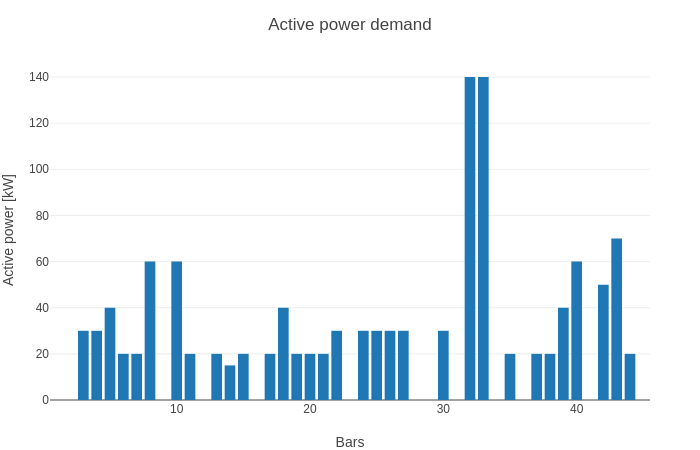
\includegraphics[width=0.7\textwidth]{7_Results/img/45fixdemand_active.png}
    \caption{Demanda de potência ativa por barra}
    \label{fig:45fixactive}
\end{figure}

\begin{figure}[H]
    \centering
    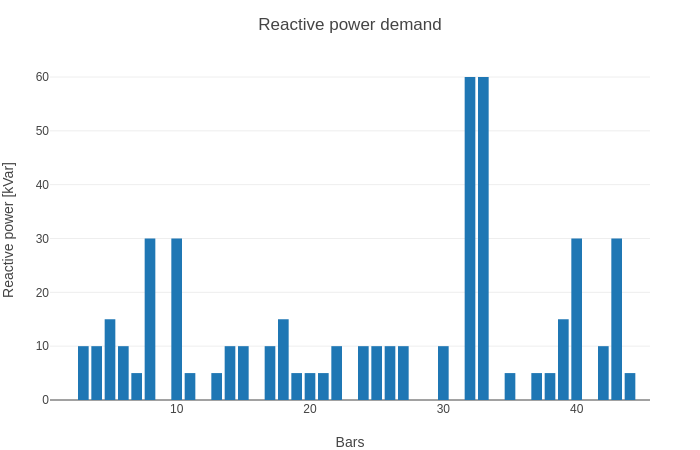
\includegraphics[width=0.7\textwidth]{7_Results/img/45fixdemand_reactive.png}
    \caption{Demanda de potência reativa por barra}
    \label{fig:45fixreactive}
\end{figure}

A partir da nova topologia, exibida na figura \ref{fig:45final}, os limites de tensões para as demandas das tabelas \ref{fig:45fixactive} e \ref{fig:45fixreactive} antes e depois da reconfiguração são dadas pelas figuras \ref{fig:45fixinitial} e \ref{fig:45fixafter} respectivamente.

\begin{figure}[H]
    \centering
    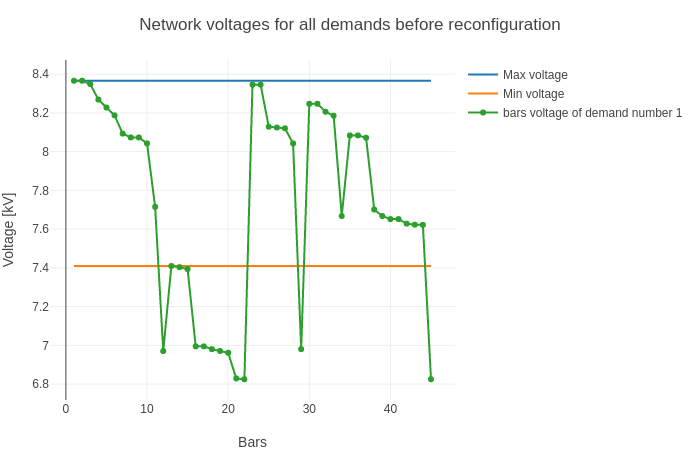
\includegraphics[width=\textwidth]{7_Results/img/45fixvoltages_before.png}
    \caption{Perfil de tensão para cada barra antes da reconfiguração}
    \label{fig:45fixinitial}
\end{figure}

\begin{figure}[H]
    \centering
    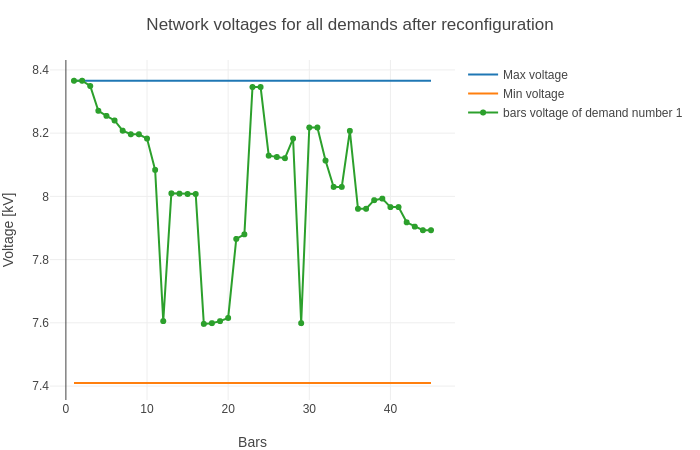
\includegraphics[width=\textwidth]{7_Results/img/45fixvoltages_after.png}
    \caption{Perfil de tensão para cada barra após a reconfiguração}
    \label{fig:45fixafter}
\end{figure}

Os dados gerais são para este perfil de demanda são dados pela tabela \ref{tab:resultsfixdemand}

\begin{table}[H]
    \centering
    \caption{Tabela de resultados para demanda fixa}
    \begin{tabular}{|c|c|c|}
    \hline
                                   & Inicial              & Reconfigurado               \\\hline
    Perdas ôhmicas por período       & \SI{613200.7}{\kilo\watt}      & \SI{369255.53}{\kilo\watt}  \\\hline
    Magnitude da tensão mínima     & \SI{6.82}{\kilo\volt}    & \SI{7.60}{\kilo\volt}   \\\hline
    Barra da tensão mínima         & 45                       & 17                      \\\hline
    Potência ativa da subestação   & \SI{1285.07}{\kilo\watt} & \SI{1257.17}{\kilo\watt}\\\hline
    Potência reativa da subestação & 495.00 kVar              & 495.17 kVar      \\\hline
    \end{tabular}
    \label{tab:resultsfixdemand}
\end{table}

Para um custo de US\$ 0.30 por kWh, o custo pré reconfiguração é de US\$ 183960,00 por ano em perdas, após a reconfiguração este custo é reduzido para US\$ 110776.00 por ano.

\subsubsection{Demanda com 3 níveis proporcionais}

\begin{figure}[H]
    \centering
    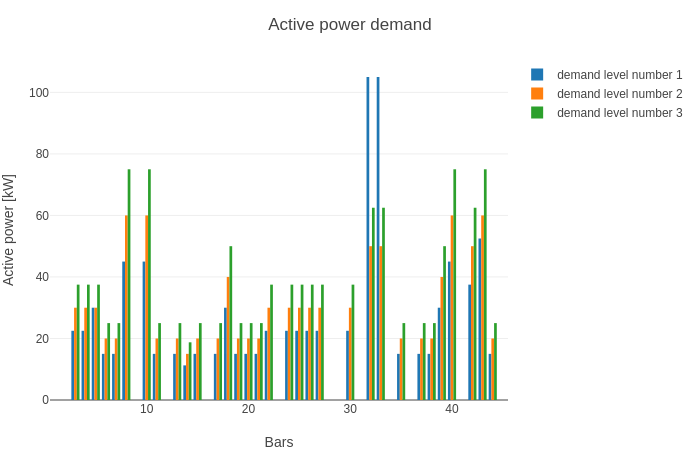
\includegraphics[width=0.8\textwidth]{7_Results/img/45demand_active.png}
    \caption{Demanda de potência ativa proporcionais a demanda média}
    \label{fig:45demandactive_propor}
\end{figure}

\begin{figure}[H]
    \centering
    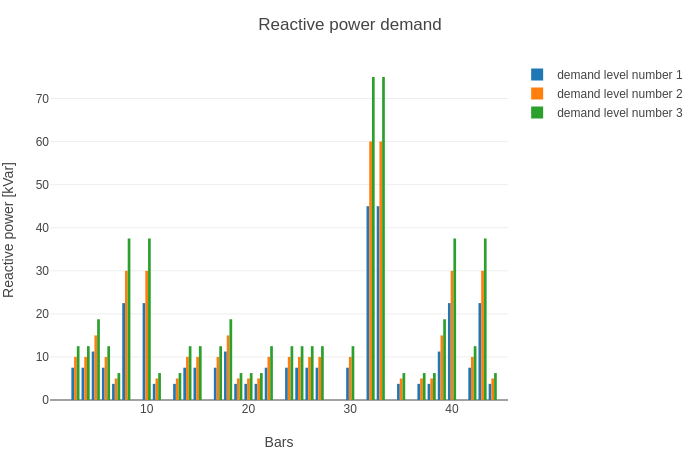
\includegraphics[width=0.8\textwidth]{7_Results/img/45demand_reactive.png}
    \caption{Demanda de potência ativa proporcionais a demanda média}
    \label{fig:45demandreactive_propor}
\end{figure}

\begin{figure}[H]
    \centering
    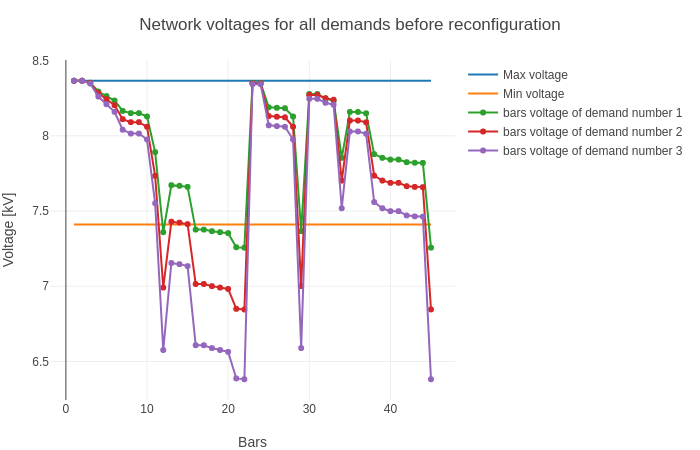
\includegraphics[width=0.8\textwidth]{7_Results/img/45voltages_before.png}
    \caption{Perfil de tensões para cada barra antes da reconfiguração}
    \label{fig:45voltages_beforesprop}
\end{figure}

\begin{figure}[H]
    \centering
    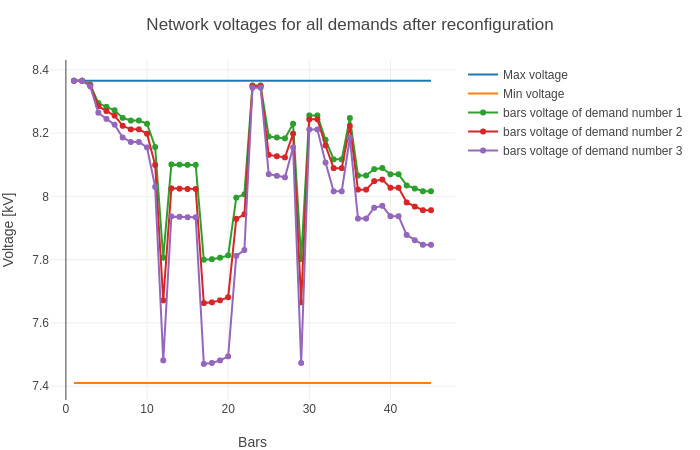
\includegraphics[width=0.8\textwidth]{7_Results/img/45voltages_after.png}
    \caption{Perfil de tensões para cada barra depois da reconfiguração}
    \label{fig:45voltaes_afterprop}
\end{figure}

\begin{table}[H]
    \centering
    \caption{Tabela de resultados para demanda 1}
    \begin{tabular}{|c|c|c|}
    \hline
                                   & Inicial              & Reconfigurado               \\\hline
    Perdas ôhmicas por período       & \SI{38768}{\kilo\watt\hour}      & \SI{23665}{\kilo\watt\hour}  \\\hline
    Magnitude da tensão mínima     & \SI{7.26}{\kilo\volt}    & \SI{7.8}{\kilo\volt}   \\\hline
    Barra da tensão mínima         & 45                       & 17                      \\\hline
    Potência ativa da subestação   & \SI{950}{\kilo\watt} & \SI{1257.17}{\kilo\watt}\\\hline
    Potência reativa da subestação & 495.00 kVar              & 495.17 kVar      \\\hline
    \end{tabular}
    \label{tab:45prop1}
\end{table}

\begin{table}[H]
    \centering
    \caption{Tabela de resultados para demanda 2}
    \begin{tabular}{|c|c|c|}
    \hline
                                   & Inicial              & Reconfigurado               \\\hline
    Perdas ôhmicas por período       & \SI{428788}{\kilo\watt\hour}      & \SI{217931}{\kilo\watt\hour}  \\\hline
    Magnitude da tensão mínima     & \SI{6.85}{\kilo\volt}    & \SI{7.66}{\kilo\volt}   \\\hline
    Barra da tensão mínima         & 45                       & 17                      \\\hline
    Potência ativa da subestação   & \SI{1078.4}{\kilo\watt} & \SI{1074.25}{\kilo\watt}\\\hline
    Potência reativa da subestação & 492.0 kVar              & 488.5 kVar      \\\hline
    \end{tabular}
    \label{tab:45prop2}
\end{table}

\begin{table}[H]
    \centering
    \caption{Tabela de resultados para demanda 3}
    \begin{tabular}{|c|c|c|}
    \hline
                                   & Inicial              & Reconfigurado               \\\hline
    Perdas ôhmicas por período       & \SI{100565.2}{\kilo\watt\hour}      & \SI{50693.4}{\kilo\watt\hour}  \\\hline
    Magnitude da tensão mínima     & \SI{6.38}{\kilo\volt}    & \SI{7.47}{\kilo\volt}   \\\hline
    Barra da tensão mínima         & 45                       & 17                      \\\hline
    Potência ativa da subestação   & \SI{1369.3}{\kilo\watt} & \SI{1319.46}{\kilo\watt}\\\hline
    Potência reativa da subestação & 624.0 kVar              & 618.3 kVar      \\\hline
    \end{tabular}
    \label{tab:45prop3}
\end{table}


Considerando um custo de US\$0.30 do kWh, antes da reconfiguração a rede, para o perfil de demanda analisado, gera um custo de aproximadamente US\$ 170436.00 devido à perdas ôhmicas em um período de 1 ano.
Após a reconfiguração, o custo devido às perdas ôhmicas é de US\$87867.00, este valor corresponde a uma redução de aproximadamente 48.5\% do valor inicial.

\subsubsection{Demanda com 4 níveis não proporcionais}

\begin{figure}[H]
    \centering
    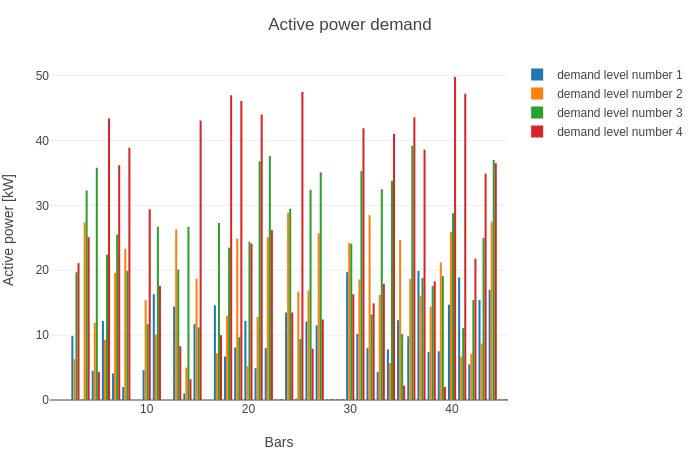
\includegraphics[width=0.8\textwidth]{7_Results/img/active_demand.png}
    \caption{Demanda de potência ativa do caso 2}
    \label{fig:45activepower2}
\end{figure}

\begin{figure}[H]
    \centering
    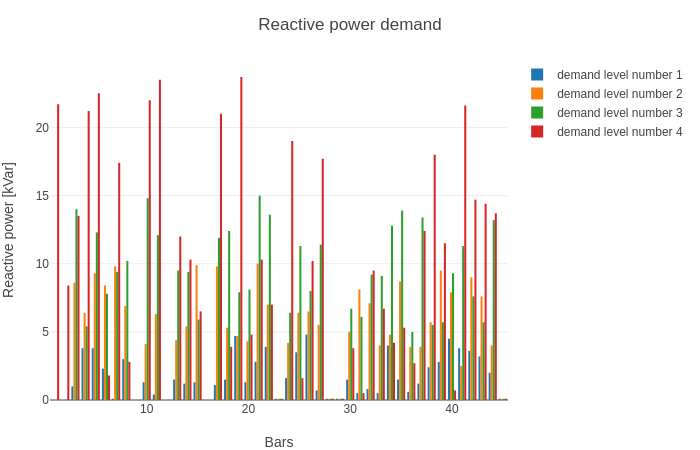
\includegraphics[width=0.7\textwidth]{7_Results/img/reactive_demand.png}
    \caption{Demanda de potência reativa do caso 2}
    \label{fig:45reactivepower2}
\end{figure}

\begin{figure}[H]
    \centering
    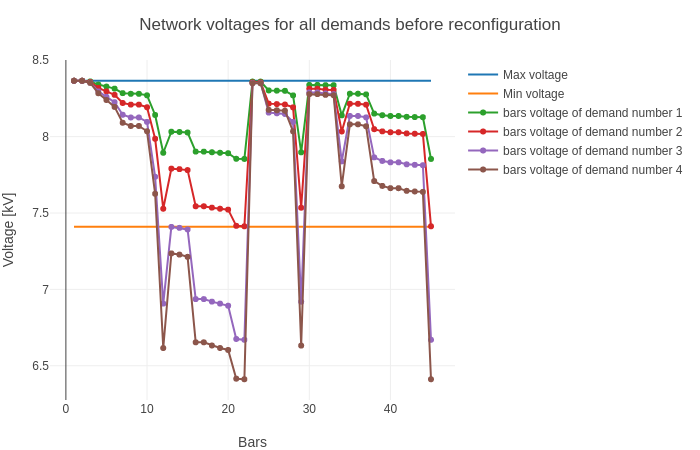
\includegraphics[width=0.9\textwidth]{7_Results/img/initial_voltages.png}
    \caption{Tensão nas barras da topologia inicial para demanda do caso 3}
    \label{fig:45voltages_init2}
\end{figure}

\begin{figure}[H]
    \centering
    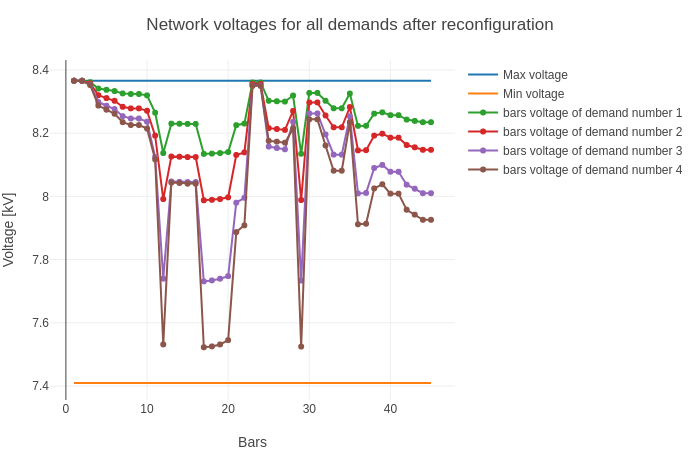
\includegraphics[width=0.9\textwidth]{7_Results/img/reconfig_voltages.png}
    \caption{Tensão nas barras após reconfiguração para demanda do caso 3}
    \label{fig:45voltages_reconfigured2}
\end{figure}

\begin{table}[H]
    \centering
    \caption{Tabela de resultados para demanda 1}
    \begin{tabular}{|c|c|c|}
    \hline
                                   & Inicial              & Reconfigurado               \\\hline
    Perdas ôhmicas por período       & \SI{7421.2}{\kilo\watt\hour}      & \SI{3817.15}{\kilo\watt\hour}  \\\hline
    Magnitude da tensão mínima     & \SI{7.85}{\kilo\volt}    & \SI{8.13}{\kilo\volt}   \\\hline
    Barra da tensão mínima         & 45                       & 17                      \\\hline
    Potência ativa da subestação   & \SI{359.9}{\kilo\watt} & \SI{355.8}{\kilo\watt}\\\hline
    Potência reativa da subestação & 82.0 kVar              & 82.0 kVar      \\\hline
    \end{tabular}
    \label{tab:45rand1}
\end{table}

\begin{table}[H]
    \centering
    \caption{Tabela de resultados para demanda 2}
    \begin{tabular}{|c|c|c|}
    \hline
                                   & Inicial              & Reconfigurado               \\\hline
    Perdas ôhmicas por período       & \SI{79273.2}{\kilo\watt\hour}      & \SI{39111.2}{\kilo\watt\hour}  \\\hline
    Magnitude da tensão mínima     & \SI{7.41}{\kilo\volt}    & \SI{7.99}{\kilo\volt}   \\\hline
    Barra da tensão mínima         & 45                       & 17                      \\\hline
    Potência ativa da subestação   & \SI{636.9}{\kilo\watt} & \SI{625.5}{\kilo\watt}\\\hline
    Potência reativa da subestação & 245.0 kVar              & 245.0 kVar      \\\hline
    \end{tabular}
    \label{tab:45rand2}
\end{table}

\begin{table}[H]
    \centering
    \caption{Tabela de resultados para demanda 3}
    \begin{tabular}{|c|c|c|}
    \hline
                                   & Inicial              & Reconfigurado               \\\hline
    Perdas ôhmicas por período       & \SI{99808.1}{\kilo\watt\hour}      & \SI{44325.2}{\kilo\watt\hour}  \\\hline
    Magnitude da tensão mínima     & \SI{6.67}{\kilo\volt}    & \SI{7.73}{\kilo\volt}   \\\hline
    Barra da tensão mínima         & 45                       & 17                      \\\hline
    Potência ativa da subestação   & \SI{936.2}{\kilo\watt} & \SI{904.5}{\kilo\watt}\\\hline
    Potência reativa da subestação & 375.0 kVar              & 370.0 kVar      \\\hline
    \end{tabular}
    \label{tab:45rand3}
\end{table}

\begin{table}[H]
    \centering
    \caption{Tabela de resultados para demanda 4}
    \begin{tabular}{|c|c|c|}
    \hline
                                   & Inicial              & Reconfigurado               \\\hline
    Perdas ôhmicas por período       & \SI{70956.8}{\kilo\watt\hour}      & \SI{32337.4}{\kilo\watt\hour}  \\\hline
    Magnitude da tensão mínima     & \SI{6.41}{\kilo\volt}    & \SI{7.52}{\kilo\volt}   \\\hline
    Barra da tensão mínima         & 45                       & 17                      \\\hline
    Potência ativa da subestação   & \SI{1057.6}{\kilo\watt} & \SI{1013.5}{\kilo\watt}\\\hline
    Potência reativa da subestação & 476.0 kVar              & 470.2 kVar      \\\hline
    \end{tabular}
    \label{tab:45rand4}
\end{table}

Com um custo de US\$ 0.30 para o kWh, para o perfil de demanda analisado, verifica-se um valor de US\$ 77237.80 antes da reconfiguração e US\$ 35877.29 para a nova topologia em um período de um ano.
\subsection{Discussão dos resultados}

Com base nos dados obtidos várias ressalvas podem ser feitas. Para a rede de 45 barras encontrou-se uma topologia que foi capaz de minimizar todos os perfis de demanda analisados para ela.
Para estes perfis houve uma redução de 45\% a 50\% nas perdas por efeito joule no sistema, de modo que em todos os perfis para todos os níveis de demanda a tensão nas barras permaneceram dentro do limite de 0.93 pu a 1.05 pu como determina a ANEEL~\cite{AgenciaNacionaldeEnergiaEletrica2018ModuloVigencia}.

\section{Conclusão}

Com este projeto foi possível observar como a reconfiguração de uma rede de distribuição de energia elétrica que opera de forma radial pode reduzir de forma considerável as perdas de potência ativa.
Além disso é possível observar como a reconfiguração do sistema de distribuição de energia elétrica manteve o nível de tensão em um intervalo determinado por norma em todas as barras do sistema.
Tensões maiores que o valor mínimo estipulado pela agência reguladora implica em uma diminuição da corrente que circula pelo conjunto de ramos do circuito de distribuição, essa redução da corrente aumenta a vida útil dos equipamentos implicando de forma indireta na redução de custo por reposição.

Esta parte do trabalho realizado mostrou que a metodologia para a transformação de um programa de PNLIM para um problema de PLIM substitui com bastante precisão o modelo não linear além de mostrar-se mais rápida e confiável, dado que modelos lineares são mais rápidos, robustos e sempre convergem em um ótimo global.

Por fim, com base nos resultados e em sua discussão, torna-se passível de discussão a ideia de distribuição de chaves ao longo dos sistemas de distribuição de energia elétrica para reconfiguração da mesma.
\section{Programação em Julia}

Há diversas vantagens em utilizar-se uma linguagem de programação como a linguagem Julia.
Uma dessas vantagens é o fato de ser gratuita, outra vantagem é a possibilidade de manipular o resultado obtendo gráficos como os que foram exibidos na seção de resultados.

O programa desenvolvido recebe estruturas de dados denominadas \emph{Dataframes}, os quais são gerados pelo programa \verb|readnetwork.jl|.

Os comandos a seguir são responsáveis por importar as bibliotecas necessárias e importar o arquivo responsável por gerar as estruturas de dados que serão usadas no problema.

\begin{lstlisting}[language = Julia]
using JuMP
using CSV
using DataFrames
using GLPK
using Blink
using PlotlyJS

#45nodes_multidemand.csv
#45nodes_network.csv
include("readnetwork.jl")
using Main.readnetwork

\end{lstlisting}

A seguir, a sequência de códigos mostra  o método usado para gerar os valores máximos dos blocos de discretização do modelo linear, bem como a inclinação dos segmentos de reta que linearizam as funções quadráticas.

\begin{lstlisting}[language = Julia,firstnumber=12]
#Parameters for PLIM formulation
mutable struct parameter
    R::Int64
    Vnom::Float64
    Vmin::Float64
    Vmax::Float64
end
plim  = parameter(50,param.Vnom[1],param.Vnom[1]*0.93,param.Vnom[1]*1.05)
dSmax = zeros(length(Ωl.num));
dSmax = plim.Vmax*Ωl.Imax/plim.R;
mS    = zeros(length(Ωl.num),plim.R);
for ol in eachrow(Ωl)
    for r in 1:plim.R
        mS[ol.num,r] = (2*r-1)*dSmax[ol.num]
    end
end
\end{lstlisting}

Comandos utilizados para definir um modelo usando o \emph{solver} \emph{GLPK} e definição das variáveis do problema de otimização.

\begin{lstlisting}[language = Julia, firstnumber = 28]
#Create a DSR optimization problem
PLIM = Model(with_optimizer(GLPK.Optimizer));
#Variables declaration
@variable(PLIM, Vqdr[Ωb.i,Ωd.num] >= 0);
@variable(PLIM, Iqdr[Ωl.num,Ωd.num] >= 0);
@variable(PLIM, PS[Ωb.i,Ωd.num]);
@variable(PLIM, QS[Ωb.i,Ωd.num]);
@variable(PLIM, Pch[Ωch.num,Ωd.num]);
@variable(PLIM, Qch[Ωch.num,Ωd.num]);
@variable(PLIM, P[Ωl.num,Ωd.num]);
@variable(PLIM, Q[Ωl.num,Ωd.num]);
@variable(PLIM, Pp[Ωl.num,Ωd.num]>=0);
@variable(PLIM, Pn[Ωl.num,Ωd.num]>=0);
@variable(PLIM, Qp[Ωl.num,Ωd.num]>=0);
@variable(PLIM, Qn[Ωl.num,Ωd.num]>=0);
@variable(PLIM, dP[Ωl.num,1:plim.R,Ωd.num]>=0);
@variable(PLIM, dQ[Ωl.num,1:plim.R,Ωd.num]>=0);
@variable(PLIM, w[Ωch.num], Bin);
\end{lstlisting}

Definição da função objetivo para redução da demanda total e fixação da barra de geração com o valor máximo de tensão bem como fixando em zero a potência de geração para as barras não geradoras.

\begin{lstlisting}[language = Julia, firstnumber = 46]
#Objective Function
@objective(PLIM, Min, cls * sum(od.T*sum(Iqdr[ol.num,od.num]*ol.R 
           for ol in eachrow(Ωl)) for od in eachrow(Ωd)));

#Define generator bar  
for od in eachrow(Ωd)    
    for ob in eachrow(Ωb)
        if ob.Tb == 1
            @constraint(PLIM, Vqdr[ob.i,od.num] == plim.Vmax^2);
        else
            @constraint(PLIM, PS[ob.i,od.num] == 0);
            @constraint(PLIM, QS[ob.i,od.num] == 0);
        end
    end
end
\end{lstlisting}

Restrição de balanço de potência para multiplas demandas.

\begin{lstlisting}[language = Julia, firstnumber = 61]
#Power balance
for od in eachrow(Ωd)    
    for ob in eachrow(Ωb)
        @constraint(PLIM, sum(P[i,od.num] for i in lines[ob.i].in) 
            - sum(P[i,od.num] + Ωl.R[i]*Iqdr[i,od.num] 
            for i in lines[ob.i].out)
            + sum(Pch[i,od.num] for i in key[ob.i].in)
            - sum(Pch[i,od.num] for i in key[ob.i].out)
            + PS[ob.i,od.num] == Ωb[!,od.P][ob.i])

        @constraint(PLIM, sum(Q[i,od.num] for i in lines[ob.i].in) 
            - sum(Q[i,od.num] + Ωl.X[i]*Iqdr[i,od.num] 
            for i in lines[ob.i].out)
            + sum(Qch[i,od.num] for i in key[ob.i].in)
            - sum(Qch[i,od.num] for i in key[ob.i].out)
            + QS[ob.i,od.num] == Ωb[!,od.Q][ob.i])
    end
end
\end{lstlisting}

Restrição de tensão entre duas barras, para diversos níveis de demanda.

\begin{lstlisting}[language = Julia, firstnumber = 77]
#Voltage between two bars
for od in eachrow(Ωd)
    for ol in eachrow(Ωl)
        @constraint(PLIM, Vqdr[ol.i,od.num] - 2(ol.R*P[ol.num,od.num] 
        + ol.X*Q[ol.num,od.num])- (ol.R^2 + ol.X^2)*Iqdr[ol.num,od.num]
        - Vqdr[ol.j,od.num] == 0)
    end
end
\end{lstlisting}

Fluxo de potência entre barras aplicas à técnica de linearização.

\begin{lstlisting}[language = Julia, firstnumber = 84]
for od in eachrow(Ωd)    
    for ol in eachrow(Ωl)
        @constraint(PLIM,plim.Vmax^2*Iqdr[ol.num,od.num] == 
            sum(dP[ol.num,r,od.num]*mS[ol.num,r] for r = 1:plim.R) 
            + sum(dQ[ol.num,r,od.num]*mS[ol.num,r] for r = 1:plim.R)) 
        @constraint(PLIM, Pp[ol.num,od.num] - Pn[ol.num,od.num] 
            == P[ol.num,od.num])
        @constraint(PLIM, Qp[ol.num,od.num] - Qn[ol.num,od.num] 
            == Q[ol.num,od.num])
        @constraint(PLIM, Pp[ol.num,od.num] + Pn[ol.num,od.num] 
            == sum(dP[ol.num,r,od.num] for r =1:plim.R))
        @constraint(PLIM, Qp[ol.num,od.num] + Qn[ol.num,od.num] 
            == sum(dQ[ol.num,r,od.num] for r =1:plim.R))
        for r=1:plim.R
            @constraint(PLIM, dP[ol.num,r,od.num] <= dSmax[ol.num])
            @constraint(PLIM, dQ[ol.num,r,od.num] <= dSmax[ol.num])
        end
    end
end
\end{lstlisting}

Aplicação da modelagem das chaves nos sistemas de interconexão.

\begin{lstlisting}[language = Julia, firstnumber = 103]
#Keys constraints
for od in eachrow(Ωd)    
    for och in eachrow(Ωch)
        @constraint(PLIM,  (plim.Vmin^2 - plim.Vmax^2)*(1-w[och.num]) 
                    <= Vqdr[och.i,od.num] - Vqdr[och.j,od.num])
        @constraint(PLIM,  Vqdr[och.i,od.num] - Vqdr[och.j,od.num] 
                    <= (plim.Vmax^2 - plim.Vmin^2)*(1-w[och.num]))
        @constraint(PLIM, -(plim.Vmax*och.Imaxch)*w[och.num] 
                    <= Pch[och.num,od.num])
        @constraint(PLIM, Pch[och.num,od.num] 
                    <= (plim.Vmax*och.Imaxch)*w[och.num])
        @constraint(PLIM, -(plim.Vmax*och.Imaxch)*w[och.num] 
                    <= Qch[och.num,od.num])
        @constraint(PLIM, Qch[och.num,od.num] 
                    <= (plim.Vmax*och.Imaxch)*w[och.num])
    end
end
\end{lstlisting}

O bloco de códigos a seguir mostra a aplicação da restrição de radialidade, limites operativos e o comando para solucionar o problema com base nas modelagens jpa descritas.

\begin{lstlisting}[language = Julia, firstnumber = 120]
#Radial constraint
@constraint(PLIM, size(Ωl,1) + sum(w[och.num] for och in eachrow(Ωch)) 
            == size(Ωb,1) - sum(Ωb.Tb));
#Voltage limits
for od in eachrow(Ωd)
    for ob in eachrow(Ωb)
        @constraint(PLIM, Vqdr[ob.i,od.num] >= plim.Vmin^2)
        @constraint(PLIM, Vqdr[ob.i,od.num] <= plim.Vmax^2)
    end
end
#Current limits
for od in eachrow(Ωd)
    for ol in eachrow(Ωl)
        @constraint(PLIM, Iqdr[ol.num,od.num] <= ol.Imax^2)
    end
end
JuMP.optimize!(PLIM)
\end{lstlisting}

O conjunto de comandos a seguir corresponde a um conjunto de aplicações usadas para exibir gráficos e estrutura de dados com os resultados obtidos.

\begin{lstlisting}[language = Julia, firstnumber = 137]
data = GenericTrace[]
for od in eachrow(Ωd)
    #push!(data,scatter(;x=Ωb.i,y=Ωb[!,od.P],mode="lines+markers",
            name=string("demand level number ", od.num)))
    push!(data,bar(;x=Ωb.i,y=Ωb[!,od.P],
            name=string("demand level number ", od.num)))
end
display(plot(data,Layout(title="Active power demand", 
            xaxis_title="Bars", yaxis_title="Active power [kW]")))
data = GenericTrace[]
for od in eachrow(Ωd)
    #push!(data,scatter(;x=Ωb.i,y=Ωb[!,od.Q],mode="lines+markers",
            name=string("demand level number ", od.num)))
    push!(data,bar(;x=Ωb.i,y=Ωb[!,od.Q],name=
            string("demand level number ",od.num)))
end
display(plot(data,Layout(title="Reactive power demand", 
            xaxis_title="Bars", yaxis_title="Reactive power [kVar]")))

#Results
obj_value_plim = JuMP.objective_value(PLIM);
Vlim  = zeros(length(Ωb.i),length(Ωd.num));   
Ilim  = zeros(length(Ωl.num),length(Ωd.num));
PSlim = zeros(length(Ωb.i),length(Ωd.num));   
QSlim = zeros(length(Ωb.i),length(Ωd.num));
Plim  = zeros(length(Ωl.num),length(Ωd.num)); 
Qlim  = zeros(length(Ωl.num),length(Ωd.num));
Pchlim  = zeros(length(Ωch.num),length(Ωd.num)); 
Qchlim  = zeros(length(Ωch.num),length(Ωd.num));

for od in eachrow(Ωd)    
    for ob in eachrow(Ωb)
        Vlim[ob.i,od.num] = sqrt(JuMP.value(Vqdr[ob.i,od.num]))
        PSlim[ob.i,od.num] = JuMP.value(PS[ob.i,od.num])
        QSlim[ob.i,od.num] = JuMP.value(QS[ob.i,od.num])
    end
end
loss_plim = Array{Float64,1}(undef,length(Ωd.num));
for od in eachrow(Ωd)
    demand_plim = 0;
    for ol in eachrow(Ωl)
        Ilim[ol.num,od.num] = sqrt(JuMP.value(Iqdr[ol.num,od.num]))
        Plim[ol.num,od.num] = JuMP.value(P[ol.num,od.num])
        Qlim[ol.num,od.num] = JuMP.value(Q[ol.num,od.num])
        demand_plim = demand_plim + ol.R*Ilim[ol.num,od.num]^2
    end
    loss_plim[od.num] = demand_plim*od.T
    for och in eachrow(Ωch)
        Pchlim[och.num,od.num] = JuMP.value(Pch[och.num,od.num])
        Qchlim[och.num,od.num] = JuMP.value(Qch[och.num,od.num])
    end

end
wlim = Int64[];
for och in eachrow(Ωch)
    push!(wlim,JuMP.value(w[och.num]))
end
vmax_plot = scatter(;x=Ωb.i,y=ones(length(Ωb.i))*plim.Vmax,
            name="Max voltage");
vmin_plot = scatter(;x=Ωb.i,y=ones(length(Ωb.i))*plim.Vmin,
            name="Min voltage");
voltages = [vmax_plot,vmin_plot]
for od in eachrow(Ωd)
    data = scatter(;x=Ωb.i,y=Vlim[:,od.num[1]],name= 
    string("bars voltage of demand number ", od.num),
    mode="lines+markers")
    push!(voltages,data)
end
display(plot(voltages,Layout(title="Network voltages for 
        all demands after reconfiguration", xaxis_title = 
        "Bars",yaxis_title = "Voltage [kV]")))
\end{lstlisting}

Aplicação da topologia inicial e módulos para exibição do resultado inicial e resultados gerais.

\begin{lstlisting}[language = Julia, firstnumber = 208]
#Create a DSR optimization problem
Init = Model(with_optimizer(GLPK.Optimizer));
#Variables declaration
@variable(Init, Vqdr[Ωb.i,Ωd.num] >= 0);
@variable(Init, Iqdr[Ωl.num,Ωd.num] >= 0);
@variable(Init, PS[Ωb.i,Ωd.num]);
@variable(Init, QS[Ωb.i,Ωd.num]);
@variable(Init, Pch[Ωch.num,Ωd.num]);
@variable(Init, Qch[Ωch.num,Ωd.num]);
@variable(Init, P[Ωl.num,Ωd.num]);
@variable(Init, Q[Ωl.num,Ωd.num]);
@variable(Init, Pp[Ωl.num,Ωd.num]>=0);
@variable(Init, Pn[Ωl.num,Ωd.num]>=0);
@variable(Init, Qp[Ωl.num,Ωd.num]>=0);
@variable(Init, Qn[Ωl.num,Ωd.num]>=0);
@variable(Init, dP[Ωl.num,1:plim.R,Ωd.num]>=0);
@variable(Init, dQ[Ωl.num,1:plim.R,Ωd.num]>=0);
@variable(Init, w[Ωch.num], Bin);

#Objective Function
@objective(Init, Min, cls * sum(od.T*sum(Iqdr[ol.num,od.num]*ol.R 
            for ol in eachrow(Ωl)) for od in eachrow(Ωd)));

#Define generator bar  
for od in eachrow(Ωd)    
    for ob in eachrow(Ωb)
        if ob.Tb == 1
            @constraint(Init, Vqdr[ob.i,od.num] == plim.Vmax^2);
        else
            @constraint(Init, PS[ob.i,od.num] == 0);
            @constraint(Init, QS[ob.i,od.num] == 0);
        end
    end
end
#Power balance
for od in eachrow(Ωd)    
    for ob in eachrow(Ωb)
        @constraint(Init, sum(P[i,od.num] for i in lines[ob.i].in) 
            - sum(P[i,od.num] + Ωl.R[i]*Iqdr[i,od.num] 
            for i in lines[ob.i].out)
            + sum(Pch[i,od.num] for i in key[ob.i].in)
            - sum(Pch[i,od.num] for i in key[ob.i].out)
            + PS[ob.i,od.num] == Ωb[!,od.P][ob.i])

        @constraint(Init, sum(Q[i,od.num] for i in lines[ob.i].in) 
            - sum(Q[i,od.num] + Ωl.X[i]*Iqdr[i,od.num] 
            for i in lines[ob.i].out)
            + sum(Qch[i,od.num] for i in key[ob.i].in)
            - sum(Qch[i,od.num] for i in key[ob.i].out)
            + QS[ob.i,od.num] == Ωb[!,od.Q][ob.i])
    end
end
#Voltage between two bars
for od in eachrow(Ωd)
    for ol in eachrow(Ωl)
        @constraint(Init, Vqdr[ol.i,od.num] - 2(ol.R*P[ol.num,od.num] 
            + ol.X*Q[ol.num,od.num])- 
            (ol.R^2 + ol.X^2)*Iqdr[ol.num,od.num] 
            - Vqdr[ol.j,od.num] == 0)
    end
end
#Piecewise linearization 
for od in eachrow(Ωd)    
    for ol in eachrow(Ωl)
        @constraint(Init,plim.Vmax^2*Iqdr[ol.num,od.num] 
            == sum(dP[ol.num,r,od.num]*mS[ol.num,r] for r = 1:plim.R) 
            + sum(dQ[ol.num,r,od.num]*mS[ol.num,r] for r = 1:plim.R)) 
        @constraint(Init, Pp[ol.num,od.num] - Pn[ol.num,od.num] 
            == P[ol.num,od.num])
        @constraint(Init, Qp[ol.num,od.num] - Qn[ol.num,od.num] 
            == Q[ol.num,od.num])
        @constraint(Init, Pp[ol.num,od.num] + Pn[ol.num,od.num] 
            == sum(dP[ol.num,r,od.num] for r =1:plim.R))
        @constraint(Init, Qp[ol.num,od.num] + Qn[ol.num,od.num] 
            == sum(dQ[ol.num,r,od.num] for r =1:plim.R))
        for r=1:plim.R
            @constraint(Init, dP[ol.num,r,od.num] <= dSmax[ol.num])
            @constraint(Init, dQ[ol.num,r,od.num] <= dSmax[ol.num])
        end
    end
end
#Keys constraints
for od in eachrow(Ωd)    
    for och in eachrow(Ωch)
        if och.ei == 0
            @constraint(Init, Pch[och.num,od.num] == 0)
            @constraint(Init, Qch[och.num,od.num] == 0)
        end
        @constraint(Init,  Vqdr[och.j,od.num] - Vqdr[och.i,od.num] 
            >= (-plim.Vmax^2)*(1-och.ei))
        @constraint(Init,  Vqdr[och.i,od.num] - Vqdr[och.j,od.num] 
            <= (plim.Vmax^2)*(1-och.ei))
    end
end
JuMP.optimize!(Init)
#Results
obj_value = JuMP.objective_value(Init);
Vinit  = zeros(length(Ωb.i),length(Ωd.num));   
Iinit  = zeros(length(Ωl.num),length(Ωd.num));
PSinit = zeros(length(Ωb.i),length(Ωd.num));   
QSinit = zeros(length(Ωb.i),length(Ωd.num));
Pinit  = zeros(length(Ωl.num),length(Ωd.num)); 
Qinit  = zeros(length(Ωl.num),length(Ωd.num));
Pchinit  = zeros(length(Ωch.num),length(Ωd.num)); 
Qchinit  = zeros(length(Ωch.num),length(Ωd.num));

for od in eachrow(Ωd)
    for ob in eachrow(Ωb)
        Vinit[ob.i,od.num] = sqrt(JuMP.value(Vqdr[ob.i,od.num]))
        PSinit[ob.i,od.num] = JuMP.value(PS[ob.i,od.num])
        QSinit[ob.i,od.num] = JuMP.value(QS[ob.i,od.num])
    end
end
loss_init = Array{Float64,1}(undef,length(Ωd.num));
for od in eachrow(Ωd)
    demand_init = 0;
    for ol in eachrow(Ωl)
        Iinit[ol.num,od.num] = sqrt(abs(JuMP.value(Iqdr[ol.num,od.num])))
        Pinit[ol.num,od.num] = JuMP.value(P[ol.num,od.num])
        Qinit[ol.num,od.num] = JuMP.value(Q[ol.num,od.num])
        demand_init = demand_init + ol.R*Iinit[ol.num,od.num]^2
    end
    loss_init[od.num] = demand_init*od.T
    for och in eachrow(Ωch)
        Pchinit[och.num,od.num] = JuMP.value(Pch[och.num,od.num])
        Qchinit[och.num,od.num] = JuMP.value(Qch[och.num,od.num])
    end
    

end
vmax_plot = scatter(;x=Ωb.i,y=ones(length(Ωb.i))*plim.Vmax,
    name="Max voltage");
vmin_plot = scatter(;x=Ωb.i,y=ones(length(Ωb.i))*plim.Vmin,
    name="Min voltage");
voltages = [vmax_plot,vmin_plot]
for od in eachrow(Ωd)
    data = scatter(;x=Ωb.i,y=Vinit[:,od.num[1]],name=
    string("bars voltage of demand number ", od.num),mode="lines+markers")
    push!(voltages,data)
end
display(plot(voltages,Layout(title="Network voltages for 
    all demands before reconfiguration",xaxis_title = 
    "Bars",yaxis_title = "Voltage [kV]")))


results = Array{DataFrame}(undef,length(Ωd.num))
for od in eachrow(Ωd)
    demand = DataFrame();
    par = ["Active power Losses [kW]", "Minimum voltage magnitude [kV]", 
        "Bar of minimum voltage magnitude",
        "Substation active power [kW]", 
        "Substation reactive power [kVar]"];
    Initial = [string(round(loss_init[od.num], digits = 2 )), 
        string(round(minimum(Vinit[:,od.num]),digits =2)),
        string(argmin(Vinit[:,od.num])), 
        string(round(maximum(PSinit[:,od.num]),digits=2)), 
        string(round(maximum(QSinit[:,od.num])))  
        ];
    
    Reconfigured = [string(round(loss_plim[od.num], digits = 2 )), 
        string(round(minimum(Vlim[:,od.num]),digits =2)),
        string(argmin(Vlim[:,od.num])), 
        string(round(maximum(PSlim[:,od.num]),digits=2)), 
        string(round(maximum(QSlim[:,od.num]),digits=2))  
        ];
    demand.Parameter = par;
    demand.Initial = Initial;
    demand.Reconfigured = Reconfigured;
    results[od.num] = demand
end

print("Cost of losses per demand period before reconfiguration: 
    US\$ ", round(JuMP.objective_value(Init),digits=2),"\n");
print("Cost of losses per demand period after  reconfiguration: 
    US\$ ", round(JuMP.objective_value(PLIM),digits=2),"\n\n");
for od in eachrow(Ωd)
    print("Demand number  ", od.num, " results:")
    print(results[od.num],"\n\n");
end

keys_states = DataFrame();
keys_states.Initial = Ωch.ei;
keys_states.Reconfigured = wlim;
print(keys_states);
\end{lstlisting}

\bibliographystyle{plain}               %Estilo de apresentação da bibliografia
\bibliography{references,webpage} %Arquivos de referência para importação

\end{document}
